%%
%% CSE407 Final Paper — ACM sigconf format
%% Upload the entire paper/ folder to Overleaf, set main.tex as the entry point.
%% Compile: pdflatex → bibtex → pdflatex → pdflatex
%% NOTE: acmart loads natbib internally — biblatex is incompatible. Use BibTeX.
%%
\documentclass[sigconf,nonacm]{acmart}

%% ── Extra packages ─────────────────────────────────────────────
\usepackage{booktabs}
\usepackage{array}
\usepackage{microtype}
\usepackage{subcaption}
\usepackage{multirow}
\usepackage{float}   %% enables [H] specifier for exact figure placement

%% ── BibTeX (acmart is incompatible with biblatex) ─────────────
%% The references.bib is authored in BibLaTeX format (url, doi, abstract,
%% eprinttype, urldate fields). BibTeX silently ignores fields it does not
%% understand and processes the standard fields (author, title, year, etc.).

%% ── BibTeX compat shim ────────────────────────────────────────
\AtBeginDocument{%
  \providecommand\BibTeX{{Bib\TeX}}}

%% ── Remove all conference / copyright metadata ─────────────────
\setcopyright{none}
\acmYear{2026}
\acmDOI{}
\acmConference[]{}{}{}
\acmISBN{}
\settopmatter{printacmref=false}  %% removes the "ACM Reference Format:" block
\setlength{\headheight}{23.5pt}
\raggedbottom

%% ── Macros ─────────────────────────────────────────────────────
\newcommand{\cmark}{\ensuremath{\checkmark}}
\newcommand{\xmark}{\ensuremath{-}}

\begin{document}

%% ════════════════════════════════════════════════════════════════
%%  TITLE AND AUTHORS
%% ════════════════════════════════════════════════════════════════
\title{Holistic Optimization of Small Language Models for Energy-Efficient Edge Inference: An Empirical Ablation Study}

\author{Md. Sadik Shahriar}
\email{shahriarsadik@gmail.com}
\affiliation{%
  \institution{East West University}
  \department{Department of Computer Science and Engineering}
  \city{Dhaka}
  \country{Bangladesh}}

\author{Nipa Mridha}
\email{mridhanipa886@gmail.com}
\affiliation{%
  \institution{East West University}
  \department{Department of Computer Science and Engineering}
  \city{Dhaka}
  \country{Bangladesh}}

\author{Tanha Humaira}
\email{chandnihumaira373@gmail.com}
\affiliation{%
  \institution{East West University}
  \department{Department of Computer Science and Engineering}
  \city{Dhaka}
  \country{Bangladesh}}

\renewcommand{\shortauthors}{Shahriar, Mridha, and Humaira}

%% ════════════════════════════════════════════════════════════════
%%  ABSTRACT
%% ════════════════════════════════════════════════════════════════
\begin{abstract}
Deploying language models on low-power devices requires cutting energy use without
destroying output quality. This paper examines what happens when three compression
methods are applied together on a real GPU: AWQ 4-bit weight quantization, a
custom PyramidKV-style token eviction scheme, and TurboQuant numerical KV-cache
quantization. We test two models---Llama~3.2-3B-Instruct and Qwen2.5-3B-Instruct---on
a single NVIDIA T4 at context lengths of 1024, 2048, and 4096 tokens. Energy is
measured from real GPU power traces sampled at 10~Hz, not estimated from formulas.
Quality is measured using a carefully designed hard-retrieval benchmark: 60 frozen
scenarios that each require the model to extract a specific code value from a
4096-token document at varying positions.

At 4096 tokens, Llama's eviction path saved 101.95~J (16.15\%) compared to its
AWQ baseline while barely affecting retrieval (37/60 vs.\ 38/60). Qwen's eviction
path saved a similar amount of energy but catastrophically dropped quality from
48/60 down to 1/60. TurboQuant's reference implementation added large energy
overhead on both models (31--45\%) because it retained extra data structures
rather than truly compressing memory. Power trace clipping tests confirmed these
findings were stable under 82~W and 70~W caps. The results show that the same
compression approach can work well on one model and completely fail on another,
and that measuring energy on real hardware gives different answers than what
published numbers might suggest.
\end{abstract}

%% ── Keywords ───────────────────────────────────────────────────
\keywords{Green AI, energy-efficient inference, KV cache compression, token
eviction, weight quantization, AWQ, TurboQuant, PyramidKV, small language models,
edge deployment, NVIDIA T4, needle-in-a-haystack}

\maketitle

%% ════════════════════════════════════════════════════════════════
%%  1. INTRODUCTION
%% ════════════════════════════════════════════════════════════════
\section{Introduction}

As language models become part of everyday applications, the energy needed to run
them becomes a real concern. Most research focuses on making models more accurate,
but less attention is paid to the power bill. When a model is used thousands of
times per day, even small inefficiencies add up to large energy costs~\cite{strubell_energy_2019,patterson_carbon_nodate,schwartz2020green}.

One of the main costs during inference (i.e., generating text from a prompt) is
the Key-Value (KV) cache. When a transformer generates tokens one at a time, it
stores information about all previous tokens in a KV cache. This cache grows
linearly as the input gets longer: more tokens means more memory reads and writes
on every single step~\cite{li2024survey}. On a small GPU like a T4, this quickly
becomes a bottleneck.

Small language models (SLMs) with fewer than 7 billion parameters are promising
for edge deployment because they use less memory~\cite{husom_sustainable_2025}.
But they still face the KV cache problem, and their energy behavior is
hardware-dependent in ways that are hard to predict without actually measuring.

There are three main approaches to compressing the KV cache and model weights:
\begin{itemize}
  \item \textbf{Weight quantization}: reduces the size of model weights.
    AWQ~\cite{lin_awq_2025} is a popular method that identifies which weights
    matter most and protects them during 4-bit compression.
  \item \textbf{Token eviction}: drops tokens from the KV cache that are judged
    unimportant. PyramidKV~\cite{cai_pyramidkv_2025} uses a pyramid-shaped budget
    across layers, keeping more tokens in early layers and fewer in later ones.
  \item \textbf{KV-cache quantization}: stores KV values in fewer bits instead of
    full FP16 precision. TurboQuant~\cite{zandieh_turboquant_2025} is a recent
    approach using random rotation and scalar codebooks.
\end{itemize}

These techniques are usually studied in isolation. We found no prior work that
measures all three together on a sub-4B model while tracking real GPU power
consumption. This study fills that gap.

The core problem is that we cannot optimize just one thing at a time. A good edge
deployment needs lower energy \emph{and} lower memory \emph{and} acceptable
output quality. These objectives sometimes conflict: a configuration that saves
the most energy might destroy output quality, making it useless in practice.

This paper studies five configurations (FP16 baseline, AWQ alone, AWQ with
eviction, AWQ with TurboQuant reference, AWQ with eviction and TurboQuant
reference) on two 3B models at three context lengths. The main question is: how
do these combinations change energy, memory, throughput, and retrieval quality on
a T4 GPU? Do the results look the same on both models?

The answers turned out to be more surprising than expected. The results show that
the same eviction method can be nearly harmless on one model and destroy the other
model's retrieval ability. TurboQuant's reference implementation actually
\emph{increased} memory usage rather than reducing it. And AWQ's energy savings
depend heavily on context length---at short prompts it can cost more. These are
the kinds of findings that only emerge from real hardware measurement.

\paragraph{Contributions.}
\begin{enumerate}
  \item Hardware energy evidence for three compression methods stacked on two
    sub-4B SLMs at three context lengths, measured from real NVML power traces.
  \item A carefully calibrated hard-retrieval benchmark and the full story of
    the three failed pilots that were needed to build it.
  \item Cross-model evidence showing that eviction results do not generalize
    between Llama and Qwen, and an analysis of what the accessible TurboQuant
    reference path actually does to memory.
  \item Pareto frontier analysis with bootstrap uncertainty showing which
    configurations are non-dominated in energy, quality, and memory simultaneously.
\end{enumerate}


%% ════════════════════════════════════════════════════════════════
%%  2. RELATED WORK
%% ════════════════════════════════════════════════════════════════
\section{Related Work}

\subsection{Weight Quantization}
Lin et al.~\cite{lin_awq_2025} developed AWQ, which works by figuring out which
model weights are most important based on activation patterns and protecting them
during 4-bit compression. Frantar et al.~\cite{frantar_gptq_2023} developed an
earlier approach (GPTQ) using second-order gradient information. Wang et
al.~\cite{wang_slmquant_2025} specifically benchmarked quantization on small
models and showed that SLMs are more sensitive to compression than large models ---
an important reason to do direct measurement on Llama and Qwen rather than
relying on large-model results.

\subsection{Token Eviction}
Zhang et al.~\cite{zhang_h2o_nodate} showed that only about 20\% of the tokens in
the KV cache are actually important (``Heavy Hitters''), meaning the rest can be
dropped. SnapKV~\cite{li_snapkv_nodate} refined this idea using a short
observation window to decide what to keep. PyramidKV~\cite{cai_pyramidkv_2025}
improved on SnapKV by using more tokens in early layers and fewer in later ones
(a pyramid shape), achieving 5--15\% better NIAH accuracy.

\subsection{KV-Cache Quantization}
Zandieh et al.~\cite{zandieh_turboquant_2025} proposed TurboQuant, which applies
a random rotation to the KV vectors, then uses an optimized scalar quantizer. The
key claim is that this works without needing calibration data. Liu et
al.~\cite{liu_kivi_2023} proposed KIVI as a 2-bit alternative. Salfati et
al.~\cite{salfati_quantization_2026} showed that quantizing KV values preserves
score ordering better than rank reduction, with growing benefits for GQA
architectures like the models tested here. Sun et al.~\cite{sun2026janusquant}
achieved accurate 2-bit quantization with JanusQuant for long-context inference.

\subsection{Combining Both Approaches}
Zhang et al.~\cite{zhang_rdkv_2026} proposed RDKV, which jointly decides how many
tokens to keep and how many bits to use per token using rate-distortion theory.
ThinKV~\cite{ramachandran_thinkv_2026} applies a similar idea to reasoning models.
These papers demonstrate the value of joint optimization, but neither provides
sub-4B T4 energy measurements. Our C4-Ref configuration stacks the two methods
sequentially and measures the interaction, which is different from the joint
optimization in RDKV.

\subsection{Energy Measurement}
Argerich et al.~\cite{argerich_watt_2026} ran over 5,000 LLM inference experiments
and established that NVML power polling at 10~Hz offers the best balance of
accuracy and overhead. They measured T4 idle power at about 12~W and peak around
82~W. Husom et al.~\cite{husom_sustainable_2025} measured quantized SLMs on edge
hardware and found that energy savings depend heavily on workload. These works
establish the measurement methodology we follow.

\subsection{Summary Table}

Table~\ref{tab:comparison} shows that no previous work combines all four
dimensions: weight quantization, token eviction, KV quantization, and real energy
measurement on sub-4B models.

\begin{table}[htbp]
\caption{Coverage Comparison with Related Work}
\label{tab:comparison}
\centering\small
\begin{tabular}{lcccc}
\toprule
\textbf{Work} & \textbf{Wt.Q} & \textbf{Evict} & \textbf{KVQ} & \textbf{Energy} \\
\midrule
AWQ~\cite{lin_awq_2025}            & \cmark & \xmark & \xmark & \xmark \\
GPTQ~\cite{frantar_gptq_2023}      & \cmark & \xmark & \xmark & \xmark \\
SLMQuant~\cite{wang_slmquant_2025} & \cmark & \xmark & \xmark & \xmark \\
H2O~\cite{zhang_h2o_nodate}        & \xmark & \cmark & \xmark & \xmark \\
SnapKV~\cite{li_snapkv_nodate}     & \xmark & \cmark & \xmark & \xmark \\
PyramidKV~\cite{cai_pyramidkv_2025}& \xmark & \cmark & \xmark & \xmark \\
TurboQuant~\cite{zandieh_turboquant_2025} & \xmark & \xmark & \cmark & \xmark \\
KIVI~\cite{liu_kivi_2023}          & \xmark & \xmark & \cmark & \xmark \\
RDKV~\cite{zhang_rdkv_2026}        & \xmark & \cmark & \cmark & \xmark \\
ThinKV~\cite{ramachandran_thinkv_2026} & \xmark & \cmark & \cmark & \xmark \\
Watt Counts~\cite{argerich_watt_2026} & \xmark & \xmark & \xmark & \cmark \\
\textbf{This Work}                 & \cmark & \cmark & \cmark & \cmark \\
\bottomrule
\end{tabular}
\end{table}


%% ════════════════════════════════════════════════════════════════
%%  3. METHODOLOGY
%% ════════════════════════════════════════════════════════════════
\section{Methodology}

As shown in Figure~\ref{fig:methodology}, the experimental pipeline combines
compression configurations, direct hardware measurements, retrieval evaluation,
and robustness analysis.

\begin{figure*}[htbp]
\centering
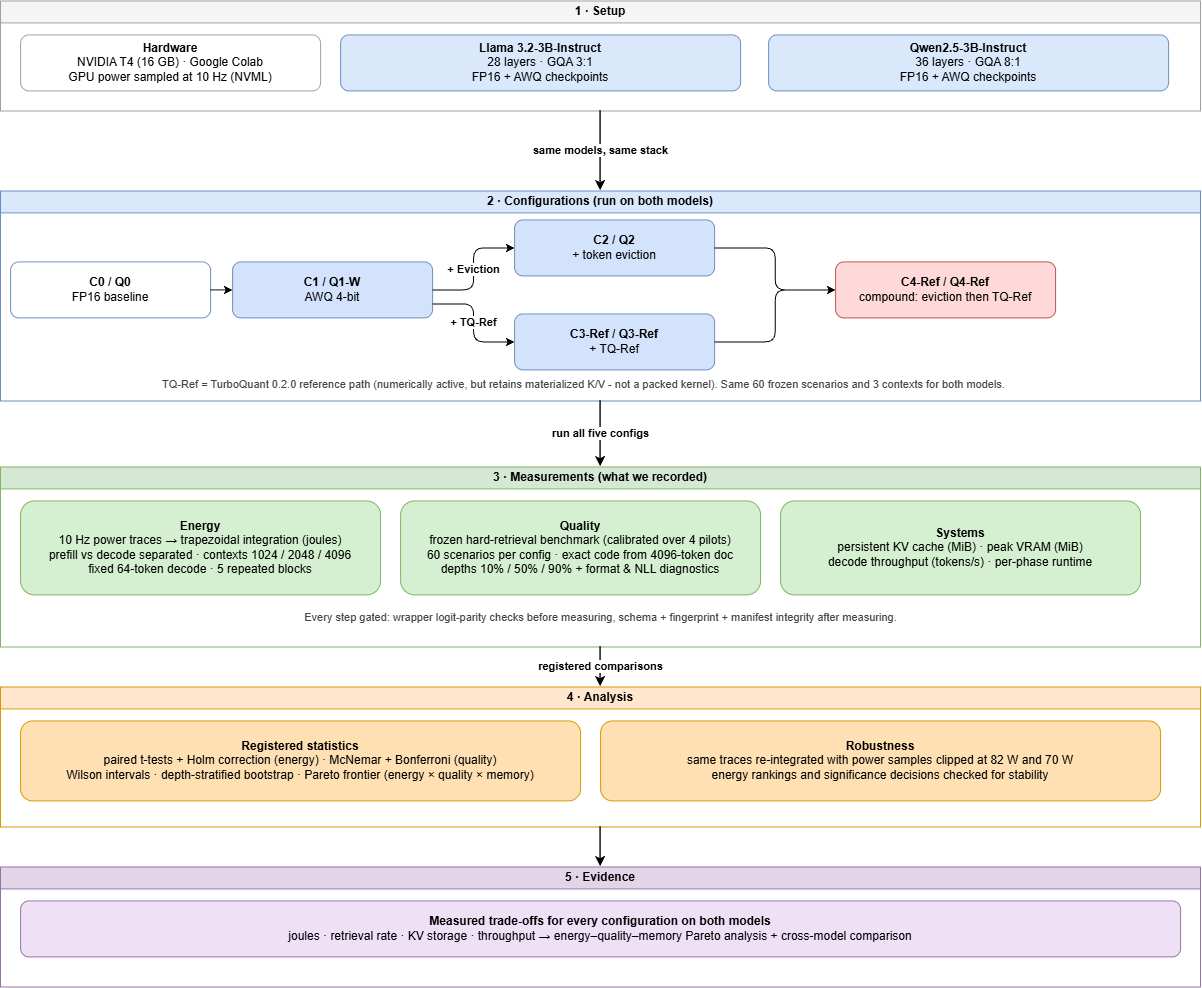
\includegraphics[width=\textwidth]{figures/methodology_diagram.png}
\Description{A flowchart summarizes the experiment: five compression configurations are evaluated on Llama 3.2-3B and Qwen2.5-3B, then power, retrieval, and system metrics are analyzed statistically and under power caps.}
\caption{Comprehensive experimental methodology flowchart. The pipeline evaluates five sequential compression configurations across two models (Llama 3.2-3B and Qwen2.5-3B), capturing physical 10 Hz power traces, hard-retrieval quality, and system trade-offs, followed by rigorous statistical and power-robustness analyses.}
\label{fig:methodology}
\end{figure*}

\subsection{Models}

We tested two small language models. Table~\ref{tab:geometry} shows their key
properties. They differ in number of layers, how their KV heads are organized
using Grouped-Query Attention (GQA)~\cite{ainslie2023gqa}, and native context window. The much more aggressive GQA ratio of
Qwen (8:1 vs.\ Llama's 3:1) is relevant for understanding why eviction behaved
so differently on the two models.

\begin{table}[htbp]
\caption{Model Architecture at a Glance}
\label{tab:geometry}
\centering\small
\begin{tabular}{lrr}
\toprule
\textbf{Property} & \textbf{Llama 3.2-3B} & \textbf{Qwen2.5-3B} \\
\midrule
Layers              & 28  & 36  \\
Query heads         & 24  & 16  \\
KV heads            & 8   & 2   \\
GQA ratio           & 3:1 & 8:1 \\
Head dimension      & 128 & 128 \\
Native context      & 8K  & 32K \\
\bottomrule
\end{tabular}
\end{table}

Llama used \texttt{unsloth/Llama-3.2-3B-Instruct}~\cite{unsloth_2024} for FP16 and the
CasperHansen AWQ release for AWQ. Qwen used the official Qwen2.5-3B-Instruct
checkpoint~\cite{qwen2024technical,qwen2024_qwen25_3b_instruct}; all revisions
were pinned in the experiment registry. We used PyTorch~2.11.0~\cite{paszke2019pytorch}
and Transformers~5.12.1~\cite{wolf2020transformers}. TurboQuant~0.2.0 was the
quantization reference implementation~\cite{zandieh_turboquant_2025,zandieh2026turboquant}.

\subsection{Configurations}

We designed five configurations to test each method individually and together:

\begin{table}[htbp]
\caption{Five Core Compression Configurations}
\label{tab:configs}
\centering\small
\resizebox{\columnwidth}{!}{%
\begin{tabular}{@{}lllll@{}}
\toprule
\textbf{Config} & \textbf{Llama} & \textbf{Qwen} & \textbf{Weights} & \textbf{KV Compression} \\
\midrule
FP16 baseline   & C0    & Q0    & FP16      & None \\
AWQ baseline    & C1/C1-W & Q1-W & AWQ 4-bit & None \\
Eviction        & C2    & Q2    & AWQ 4-bit & PyramidKV-style token eviction \\
TQ-Ref only     & C3-Ref & Q3-Ref & AWQ 4-bit & TurboQuant numerical reference \\
Compound        & C4-Ref & Q4-Ref & AWQ 4-bit & Eviction \emph{then} TQ-Ref \\
\bottomrule
\end{tabular}}
\end{table}

Two sensitivity sweeps were also run at 4096 tokens: eviction budget (512, 1024,
1536 average retained tokens per layer) and TQ nominal bit width (2, 3, 4).

\subsection{Hardware and Energy Measurement}

All experiments ran on a single NVIDIA T4 (16~GB) in Google Colab free tier.
GPU power was sampled every 100~ms (10~Hz) using NVML~\cite{nvidia2024nvml} via pynvml, following the
methodology of Argerich et al.~\cite{argerich_watt_2026}. Energy was computed as
the area under the power curve (trapezoidal integration) and reported separately
for prefill and decode phases.

We used a fixed 64-token teacher-forced decode for reproducibility: the model
always generates the same output sequence regardless of configuration, so any
energy difference is purely from the compression path. Contexts were 1024, 2048,
and 4096 tokens. Five energy blocks were collected per condition.

All power traces, timestamps, GPU clock state, temperature, and allocated VRAM
were saved. This allowed us to later reintegrate the same traces with power
spikes clipped (see Section~\ref{sec:robustness}).

\subsection{The Eviction Implementation}

Our eviction uses a custom attention wrapper. At each layer, attention scores from
the last 32 tokens are pooled to build an importance score for all past tokens.
A pyramidal budget is applied across layers: deeper layers keep more tokens and
shallower layers keep fewer, averaging 1024 tokens per layer. At every prefill,
the bottom-scoring tokens are removed and their key-value states are freed. This
is the same idea as PyramidKV, but implemented from scratch so that every step
could be validated.

For Qwen, the wrapper was verified separately on its 8:1 GQA geometry before any
measurements were collected (Section~\ref{sec:adapter}).

\subsection{The TurboQuant Reference Path}

TurboQuant~\cite{zandieh_turboquant_2025,zandieh2026turboquant} applies a random rotation to KV vectors
and then quantizes each coordinate with an optimized scalar codebook. We used
version~0.2.0~\cite{zandieh2026turboquant}. At this version, the implementation stores one uint8 index per
coordinate and \emph{keeps} the original (materialized) K/V tensors alongside
the quantization state. This means the reference path is numerically active ---
the compressed indices do affect computations --- but it does not reduce memory
because the original tensors are still resident. The bit-width setting (2, 3, or
4 bits) controls codebook resolution, not physical storage format.

This distinction is critical for interpreting our results: TQ-Ref shows what the
quantization \emph{numerics} do, but not what a fully optimized packed
implementation would achieve.

\subsection{Statistical Analysis}

Registered energy comparisons used paired $t$-tests on five common blocks, with
95\% confidence intervals and Holm sequential correction~\cite{holm1979simple}. Hard retrieval quality
used Wilson score intervals~\cite{wilson1927probable} at 60 scenarios per configuration and Bonferroni-adjusted
exact McNemar tests~\cite{mcnemar1947note} for paired comparisons. Wilcoxon signed-rank tests~\cite{wilcoxon1945individual}
were used for non-parametric energy comparisons. Cross-model quality contrasts used
depth-stratified bootstrap resampling with 2000 iterations. Pareto frontier
stability was assessed with 2000 bootstrap resamples of the empirical points.


%% ════════════════════════════════════════════════════════════════
%%  4. DESIGNING THE HARD-RETRIEVAL BENCHMARK
%% ════════════════════════════════════════════════════════════════
\section{Designing the Retrieval Benchmark}
\label{sec:benchmark}

This section explains how we built the quality benchmark, including the three
attempts that failed before we got a working design.

\subsection{Why We Needed a New Benchmark}

Early Llama experiments used a simple needle-in-a-haystack~\cite{kamradt2023needle} task where the model
had to find one code value hidden in a document. The problem was that all five
configurations got 100\% accuracy. That looks great, but it actually means the
task was too easy --- we could not tell which method was better or worse because
they all succeeded every time.

We therefore designed a harder task: the model must find and extract an exact code
value that appears at a specific position in a 4096-token document, and both the
answer format and the value must be exactly right. Three depths were tested: near
the beginning (10\%), middle (50\%), and near the end (90\%) of the document.

\subsection{Three Failed Attempts}

\paragraph{Pilot V1 --- Too Many Confusing Records.}
The first version had 48 records in the document. Both the AWQ baseline (C1-W)
and the eviction path (C2) got 6 out of 12 right. The problem: the task was too
hard for both. Many records had similar-looking codes, and the model kept
retrieving the wrong one. When baseline and treatment fail at the same rate, you
cannot tell whether compression made things worse.

\paragraph{Pilot V2 --- Fewer Records Did Not Help.}
We reduced the document to 32 records. Results were the same: 6/12 for both
paths. The confusion was not about record count but about similar-looking values.

\paragraph{Pilot V3 --- Close Siblings Made It Worse.}
We tried adding ``close siblings''---records with very similar codes to create
harder discrimination. This backfired. C1-W fell to 3/12 and C2 to 2/12. At
50\% and 90\% depths, neither configuration got a single correct answer. This
taught a key lesson: \emph{a benchmark where the baseline mostly fails cannot
diagnose compression effects}. The baseline needs to succeed often enough that a
compression method that hurts quality will clearly show up.

\paragraph{Pilot V4 --- Calibrated and Frozen.}
The fourth design used simpler, more distinctive records with unique node names
that reduced visual confusion. C1-W scored 9/12 and C2 scored 9/12. This passed
our minimum-headroom requirement: the baseline succeeded well enough, and there
was room to observe a drop if eviction damaged retrieval. We froze the prompt
design and expanded it to 60 scenarios per configuration (20 at each depth).

The V4 rows themselves were \emph{not} counted as final evidence because they
influenced the benchmark design. All pilot data is stored separately and excluded
from quality estimates.

\subsection{The Final Frozen Benchmark}

The frozen benchmark has exactly 60 scenarios per configuration. Each scenario is
tokenized independently by each model, and the document is padded to exactly 4096
tokens. The model must output the target code exactly (same format and value) to
count as correct. Retrieval correctness and format correctness are scored
separately. We report retrieval (finding the correct value) as the primary metric.

The same 60 scenarios were used for Llama and Qwen, but each model produced its
own tokenized 4096-token version using its own tokenizer and chat template.

As shown in Figure~\ref{fig:hard_retrieval}, the target code appears at one of
three controlled depths within each otherwise distractor-filled document.

\begin{figure*}[!t]
\centering
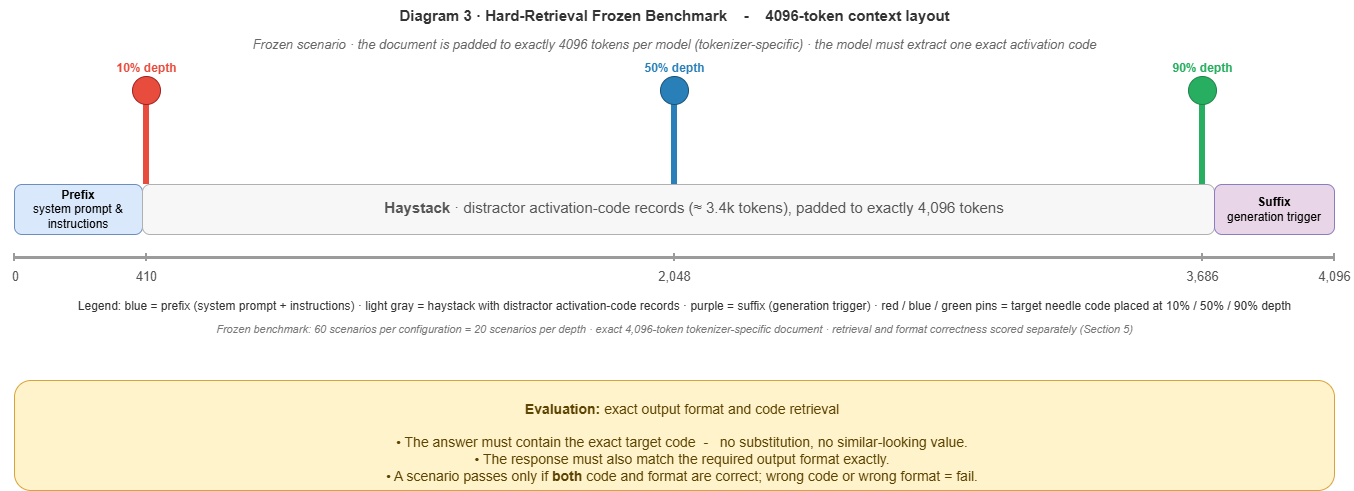
\includegraphics[width=0.98\textwidth]{figures/hard_retrieval.png}
\Description{A 4096-token document diagram shows target-code needles inserted at 10, 50, and 90 percent depth within distractor text, with strict exact-match evaluation.}
\caption{Overview of the 4096-token frozen hard-retrieval benchmark, illustrating the 10\%, 50\%, and 90\% depth needle insertion points within the distractor haystack, and the strict evaluation criteria.}
\label{fig:hard_retrieval}
\end{figure*}


%% ════════════════════════════════════════════════════════════════
%%  5. RESULTS
%% ════════════════════════════════════════════════════════════════
\section{Results}

We first report the measured energy and system trade-offs, then assess retrieval
quality, cross-model behavior, and robustness to power-trace clipping.

\subsection{TurboQuant Reference Energy Overhead by Phase}

\begin{figure*}[htbp]
\centering
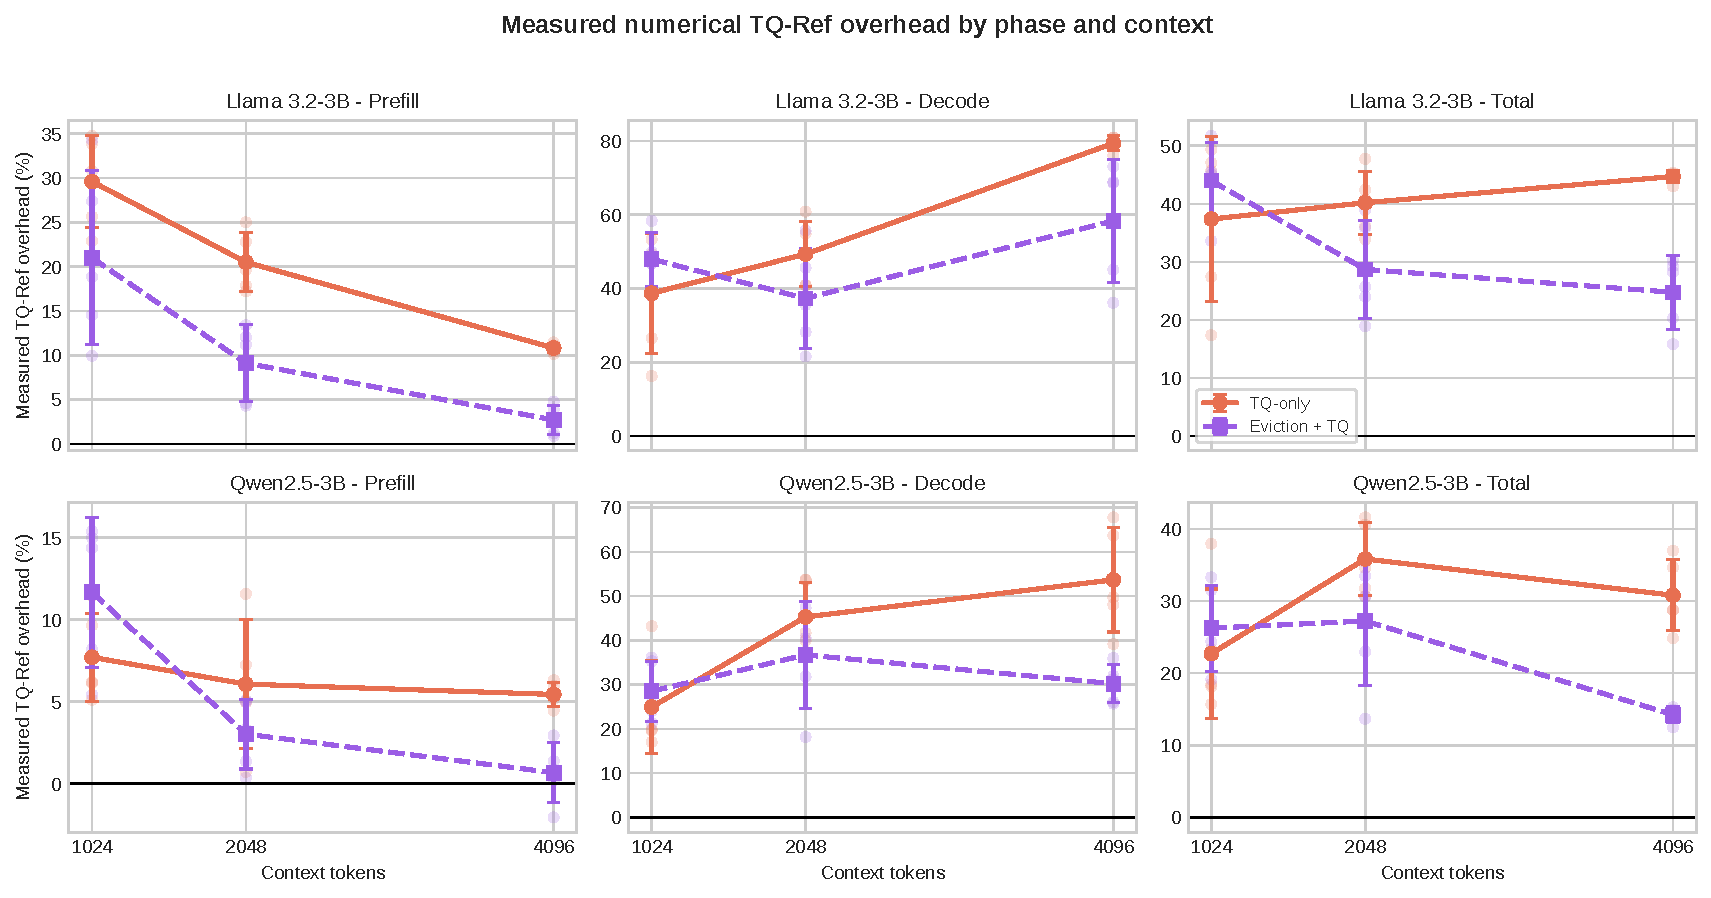
\includegraphics[width=\textwidth]{figures/fig01_measured_tq_overhead.pdf}
\Description{Bar charts compare the TQ-Ref energy overhead during prefill, decode, and total inference across three context lengths for Llama and Qwen.}
\caption{Measured TQ-Ref energy overhead (\%) relative to the matched non-TQ
baseline, split by prefill, decode, and total energy, for both models at 1024,
2048, and 4096 context tokens. Filled circles = TQ-only; dashed squares =
Eviction~+~TQ. All plotted mean overheads remain above zero. At 4096, Llama
TQ-only total overhead reaches $\approx$45\% (decode overhead $\approx$80\%);
eviction reduces Llama compound overhead to $\approx$25\%. Qwen compound
overhead falls to $\approx$14\%.}
\label{fig:tq-overhead}
\end{figure*}

Figure~\ref{fig:tq-overhead} makes the TQ-Ref overhead immediately visible. All
mean overheads are positive across both models and all three contexts: the
reference implementation consistently adds energy. The decode overhead grows
fastest with context (reaching $\approx$80\% for Llama TQ-only at 4096 tokens)
because the decode phase does proportionally more reads of the growing cache.
Eviction reduces compound overhead because it shrinks the cache before TQ-Ref
operates on it --- the shielding effect analyzed in Section~\ref{sec:interaction}.

\subsection{Llama: Energy Across Context Lengths}
\label{sec:llama-energy}

Table~\ref{tab:llama-all} shows the measured energy and throughput for all five
Llama configurations at all three context lengths.

\begin{table}[htbp]
\caption{Llama Energy (J, mean $\pm$ SD) and Throughput at All Contexts}
\label{tab:llama-all}
\centering\small
\resizebox{\columnwidth}{!}{%
\begin{tabular}{@{}lrrrr@{}}
\toprule
\textbf{Config@Context} & \textbf{Total J} & \textbf{tok/s} & \textbf{Peak VRAM (MiB)} & \textbf{Cache (MiB)} \\
\midrule
C0 @ 1024   & $244.11 \pm 13.10$ & 21.09 & 8810 & 119 \\
C1 @ 1024   & $268.77 \pm 26.20$ & 18.24 & 4943 & 119 \\
C2 @ 1024   & $253.61 \pm 14.36$ & 19.31 & 4920 & 92  \\
C3 @ 1024   & $367.00 \pm 28.44$ & 13.49 & 5099 & 187 \\
C4 @ 1024   & $364.91 \pm 21.59$ & 12.75 & 5042 & 147 \\
\midrule
C0 @ 2048   & $345.26 \pm 4.97$  & 17.42 & 9663 & 231 \\
C1 @ 2048   & $313.81 \pm 9.31$  & 20.13 & 5795 & 231 \\
C2 @ 2048   & $338.74 \pm 21.03$ & 17.81 & 5691 & 119 \\
C3 @ 2048   & $439.58 \pm 9.11$  & 13.33 & 6116 & 357 \\
C4 @ 2048   & $435.05 \pm 24.47$ & 12.87 & 5853 & 187 \\
\midrule
C0 @ 4096   & $701.08 \pm 8.12$  & 11.34 & 12688 & 455 \\
C1 @ 4096   & $631.25 \pm 5.05$  & 13.77 & 8820  & 455 \\
C2 @ 4096   & $529.30 \pm 20.02$ & 20.34 & 8500  & 119 \\
C3 @ 4096   & $913.48 \pm 2.11$  & 7.66  & 9468  & 697 \\
C4 @ 4096   & $659.50 \pm 21.35$ & 12.53 & 8662  & 187 \\
\bottomrule
\end{tabular}}
\end{table}

\begin{figure*}[htbp]
\centering
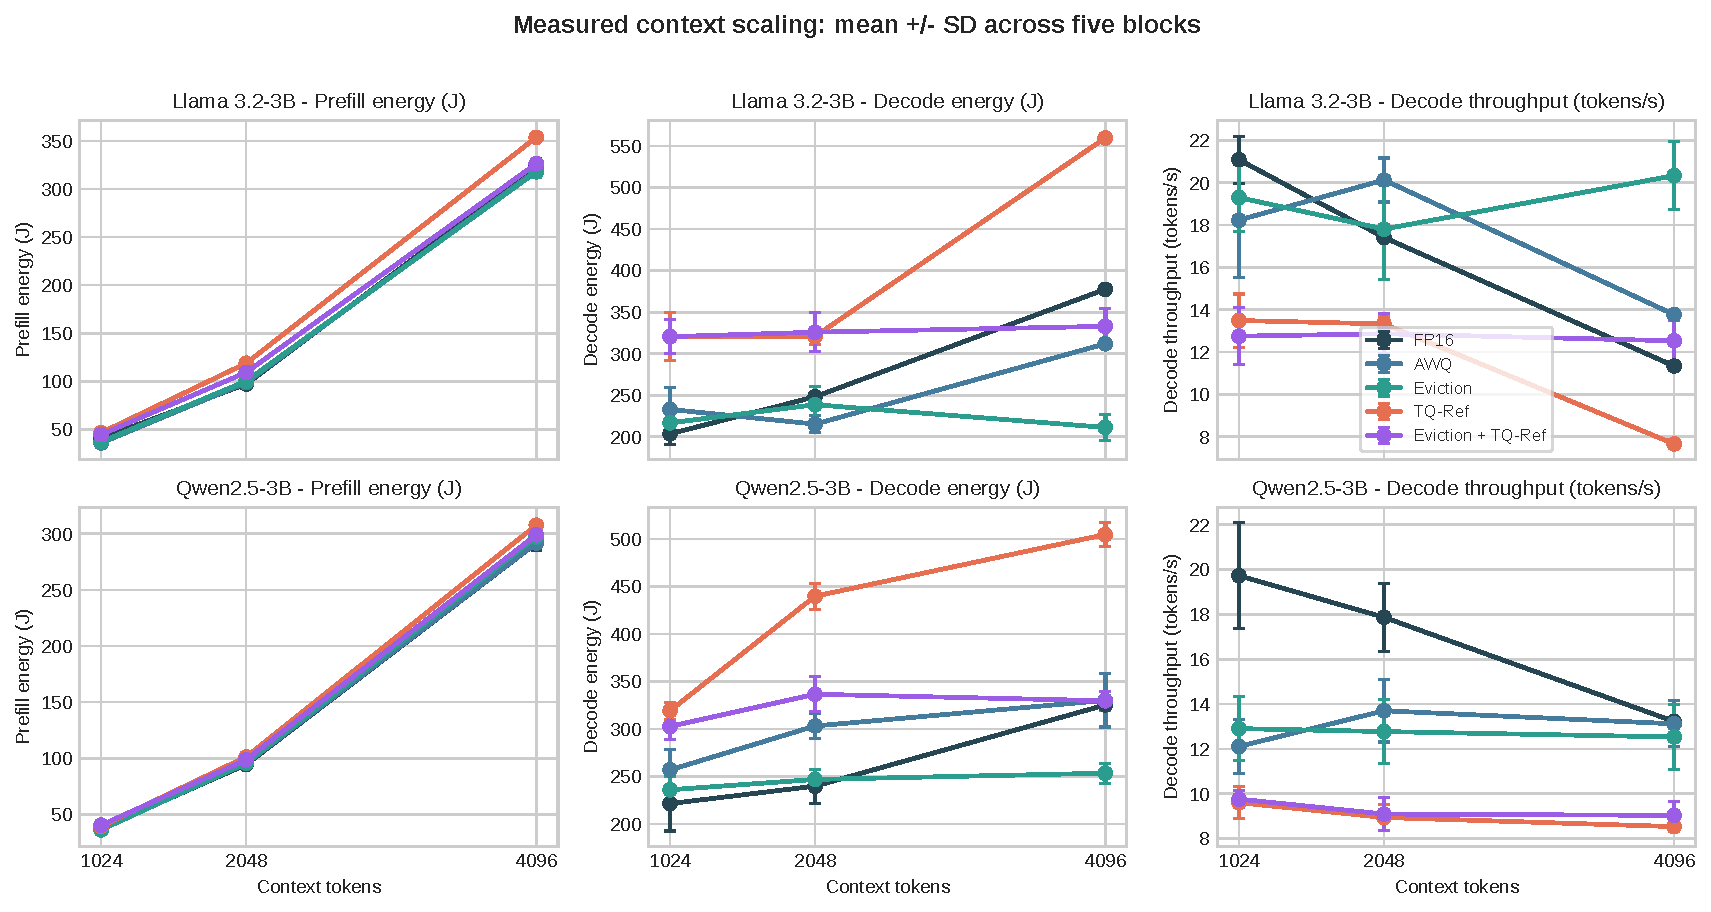
\includegraphics[width=\textwidth]{figures/fig02_measured_context_scaling.pdf}
\Description{Three plots show prefill energy, decode energy, and decode throughput by context length and compression configuration for both models.}
\caption{Measured context scaling for both models: prefill energy (left), decode
energy (center), and decode throughput (right) at 1024, 2048, and 4096 context
tokens. Prefill differences are small across configurations because full-prompt
attention runs before compression takes effect. The largest differences appear in
decode: eviction (Eviction) lowers decode energy and raises throughput at long
context; TQ-Ref raises decode energy and lowers throughput.}
\label{fig:context-scaling}
\end{figure*}

A few patterns stand out from Table~\ref{tab:llama-all} and
Figure~\ref{fig:context-scaling}:

\textbf{AWQ energy depends on context.} At 1024 tokens, AWQ (C1) used
\emph{more} energy than FP16 (C0): 268.77~J vs.\ 244.11~J. At 4096, C1 used
about 10\% less: 631.25~J vs.\ 701.08~J. AWQ is not always cheaper; its benefit
grows with context length.

\textbf{Eviction helps most at long context.} At 4096 tokens, C2 saved 101.95~J
(16.15\%) compared to C1. Decode throughput jumped from 13.77 to 20.34 tokens/s
--- C2 decoded nearly 48\% faster. The live KV cache shrank from 455~MiB to
119~MiB (73.8\% less). At 1024 tokens, the eviction budget barely changed the
cache size and the energy saving was small.

\textbf{TQ-Ref is the most expensive path.} C3 used 913.48~J at 4096 tokens ---
44.7\% more than C1. Its throughput dropped to 7.66 tokens/s (roughly half of C1)
and its cache grew to 697~MiB (bigger than the FP16 baseline at 455~MiB).

\textbf{The compound path sits in between.} C4 used 659.50~J at 4096 tokens, only
28.26~J above C1. Prior eviction reduced the cache size before TQ-Ref operated
on it, which is why C4 is cheaper than C3.

\subsection{Llama: Statistical Tests at 4096 Tokens}

Table~\ref{tab:llama-stats} shows the formal paired test results. The C1-vs-C2
difference was statistically significant after Holm correction ($p = 0.00549$),
as was the large C1-vs-C3 penalty. C1 and C4 did not differ significantly
($p = 0.2465$). This does not mean they are exactly equal; it means five blocks
were not enough to resolve the 28~J gap with certainty.

\begin{table}[htbp]
\caption{Registered Paired Tests at 4096 Tokens, Llama Total Energy}
\label{tab:llama-stats}
\centering\small
\resizebox{\columnwidth}{!}{%
\begin{tabular}{@{}lrrrl@{}}
\toprule
\textbf{Comparison} & \textbf{Diff (J)} & \textbf{95\% CI (J)} & \textbf{Holm p} & \textbf{Decision} \\
\midrule
C1 $-$ C2     & $+101.95$ & $[73.81,\ 130.08]$    & 0.00549  & C2 lower; significant \\
C1 $-$ C3-Ref & $-282.24$ & $[-287.23,\ -277.25]$ & $1.9\!\times\!10^{-7}$ & C3 much higher \\
C1 $-$ C4-Ref & $-28.26$  & $[-60.28,\ 3.76]$     & 0.2465   & Not significant \\
C2 $-$ C4-Ref & $-130.21$ & $[-168.32,\ -92.09]$  & 0.00620  & C4 higher \\
C3 $-$ C4-Ref & $+253.98$ & $[226.93,\ 281.02]$   & 0.000206 & C4 lower \\
\bottomrule
\end{tabular}}
\end{table}

\subsection{Sequential Interaction: Does Eviction Shield TQ-Ref Overhead?}
\label{sec:interaction}

When eviction runs first and then TQ-Ref operates on the smaller cache (C4), is
the energy overhead the same as doing TQ-Ref on the full cache (C3)? We measured:
\begin{equation}
I = (\text{C4} - \text{C3}) - (\text{C2} - \text{C1})
\end{equation}
A negative $I$ means eviction \emph{reduced} TQ-Ref overhead. For Llama,
$I = -152.03$~J (95\% CI: $[-187.11, -116.96]$, $p = 0.00109$). This significant
shielding effect confirms that eviction shrank the cache before TQ-Ref, reducing
the work done. However, C4 was still 130.21~J more expensive than C2 alone ---
eviction made TQ-Ref cheaper, not free.

\begin{figure}[htbp]
\centering
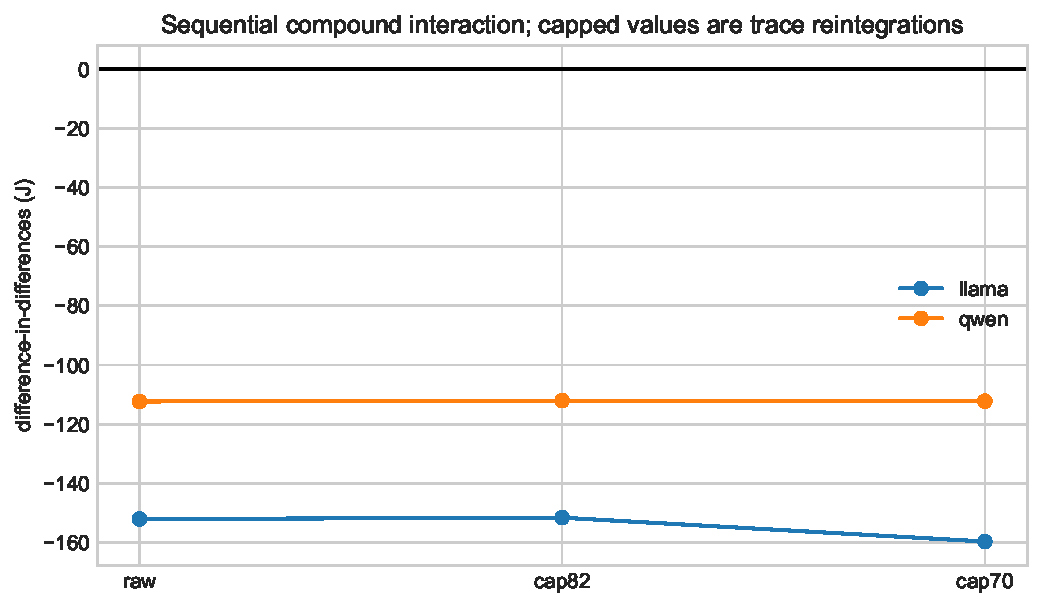
\includegraphics[width=\columnwidth]{figures/fig_interaction_by_power_regime.pdf}
\Description{A grouped bar chart shows negative eviction--TQ interaction values for Llama and Qwen under raw, 82-watt-capped, and 70-watt-capped power traces.}
\caption{Sequential compound interaction ($I$) for Llama (left, orange) and Qwen
(right, blue) under raw, 82~W-capped, and 70~W-capped trace integration. Both
values remain below zero (negative $I$ = eviction shields TQ overhead) and are
stable across all three power regimes.}
\label{fig:interaction}
\end{figure}

Figure~\ref{fig:interaction} confirms that the same negative interaction held for
Qwen, and that both results were stable when power-trace clipping was applied.

\subsection{Llama: System Trade-Offs at 4096 Tokens}

\begin{figure}[htbp]
\centering
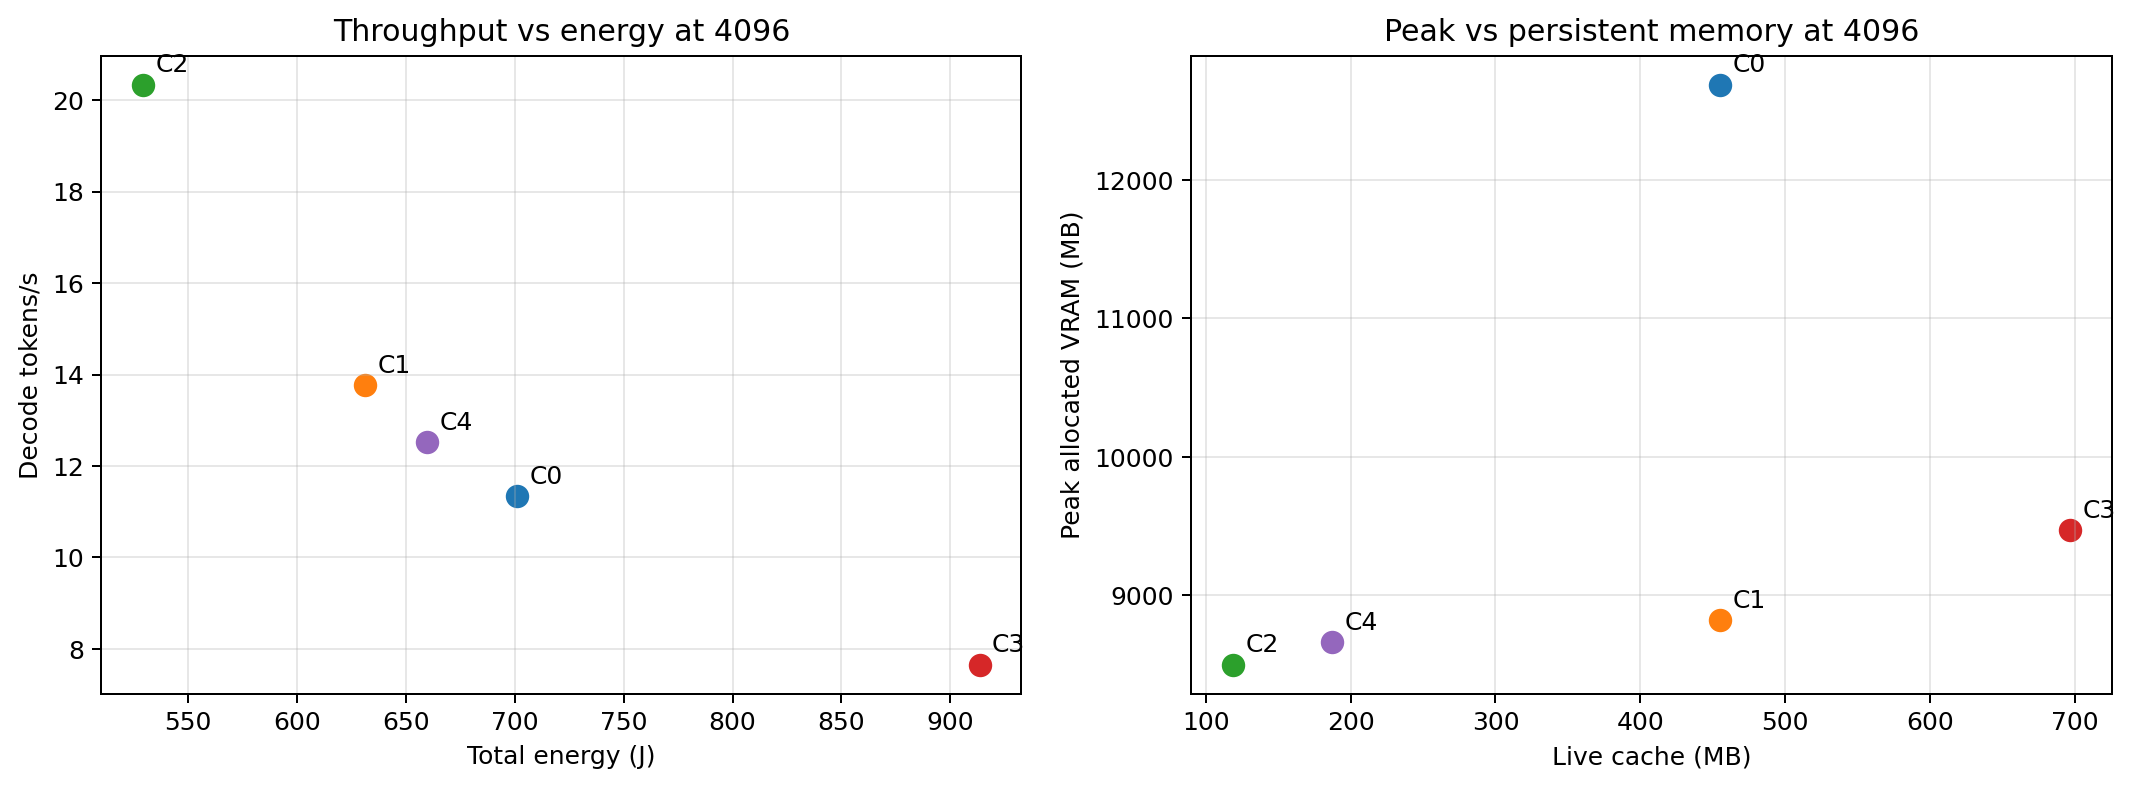
\includegraphics[width=\columnwidth]{figures/v5_final_system_tradeoffs_4096.png}
\Description{Two scatter plots compare Llama throughput with energy and peak VRAM with live cache size at 4096 tokens.}
\caption{Left: throughput vs.\ total energy for Llama at 4096 tokens. C2 is best
on both axes: lowest energy and highest throughput. Right: peak allocated VRAM vs.\
live cache. C3 has both the highest peak VRAM and the largest live cache; C2 has
the smallest.}
\label{fig:tradeoffs}
\end{figure}

Figure~\ref{fig:tradeoffs} shows the trade-offs from two angles. The left panel
confirms C2 is clearly best for energy-per-throughput. The right panel shows C3's
memory overhead is real: it has both a large live cache (697~MiB) and the highest
peak VRAM, while C2 achieves both small live cache (119~MiB) and low peak VRAM.

\subsection{Llama: Hard-Retrieval Quality Results}

Table~\ref{tab:llama-quality} shows the hard-retrieval results from the frozen
60-scenario benchmark. All rates include Wilson 95\% confidence intervals.

\begin{table}[htbp]
\caption{Llama Hard-Retrieval at 4096 Tokens (60 Scenarios)}
\label{tab:llama-quality}
\centering\small
\begin{tabular}{lrrl}
\toprule
\textbf{Config} & \textbf{Pass/60} & \textbf{Rate} & \textbf{Wilson 95\% CI} \\
\midrule
C0 (FP16)     & 47/60 & 0.783 & $[0.664,\ 0.869]$ \\
C1-W (AWQ)    & 38/60 & 0.633 & $[0.507,\ 0.744]$ \\
C2 (Evict)    & 37/60 & 0.617 & $[0.490,\ 0.729]$ \\
C3-Ref (TQ)   & 37/60 & 0.617 & $[0.490,\ 0.729]$ \\
C4-Ref (Both) & 37/60 & 0.617 & $[0.490,\ 0.729]$ \\
\bottomrule
\end{tabular}
\end{table}

FP16 (C0) was clearly better than AWQ paths on this hard task. However, the three
AWQ-with-compression paths (C2, C3-Ref, C4-Ref) each differed from the AWQ
baseline (C1-W) by \emph{only one scenario} out of 60. The failure mode was
mostly ``wrong code'' --- the model retrieved a plausible-looking value that was
not the target, rather than returning nothing.

Table~\ref{tab:depth} shows results by depth. All configurations did best at 10\%
(near the start) and worse at 50\% and 90\%.

\begin{table}[htbp]
\caption{Llama Retrieval by Document Depth}
\label{tab:depth}
\centering\small
\begin{tabular}{lrrr}
\toprule
\textbf{Config} & \textbf{10\%} & \textbf{50\%} & \textbf{90\%} \\
\midrule
C0     & 19/20 & 13/20 & 15/20 \\
C1-W   & 18/20 & 10/20 & 10/20 \\
C2     & 18/20 & 10/20 &  9/20 \\
C3-Ref & 18/20 & 10/20 &  9/20 \\
C4-Ref & 17/20 & 10/20 & 10/20 \\
\bottomrule
\end{tabular}
\end{table}

\subsection{Pareto Frontier with Uncertainty}

The measured three-objective Pareto frontier (raw total energy, hard retrieval,
persistent KV bytes) at 4096 tokens is shown in Table~\ref{tab:pareto3}, with
bootstrap frontier-selection frequency over 2000 resamples.
Figure~\ref{fig:pareto3obj} shows the same measured points: marker area encodes
persistent KV storage (bigger~=~more memory), horizontal bars show energy SD,
vertical bars show Wilson quality intervals, and edge width encodes bootstrap
frontier-selection stability.

\begin{figure*}[htbp]
\centering
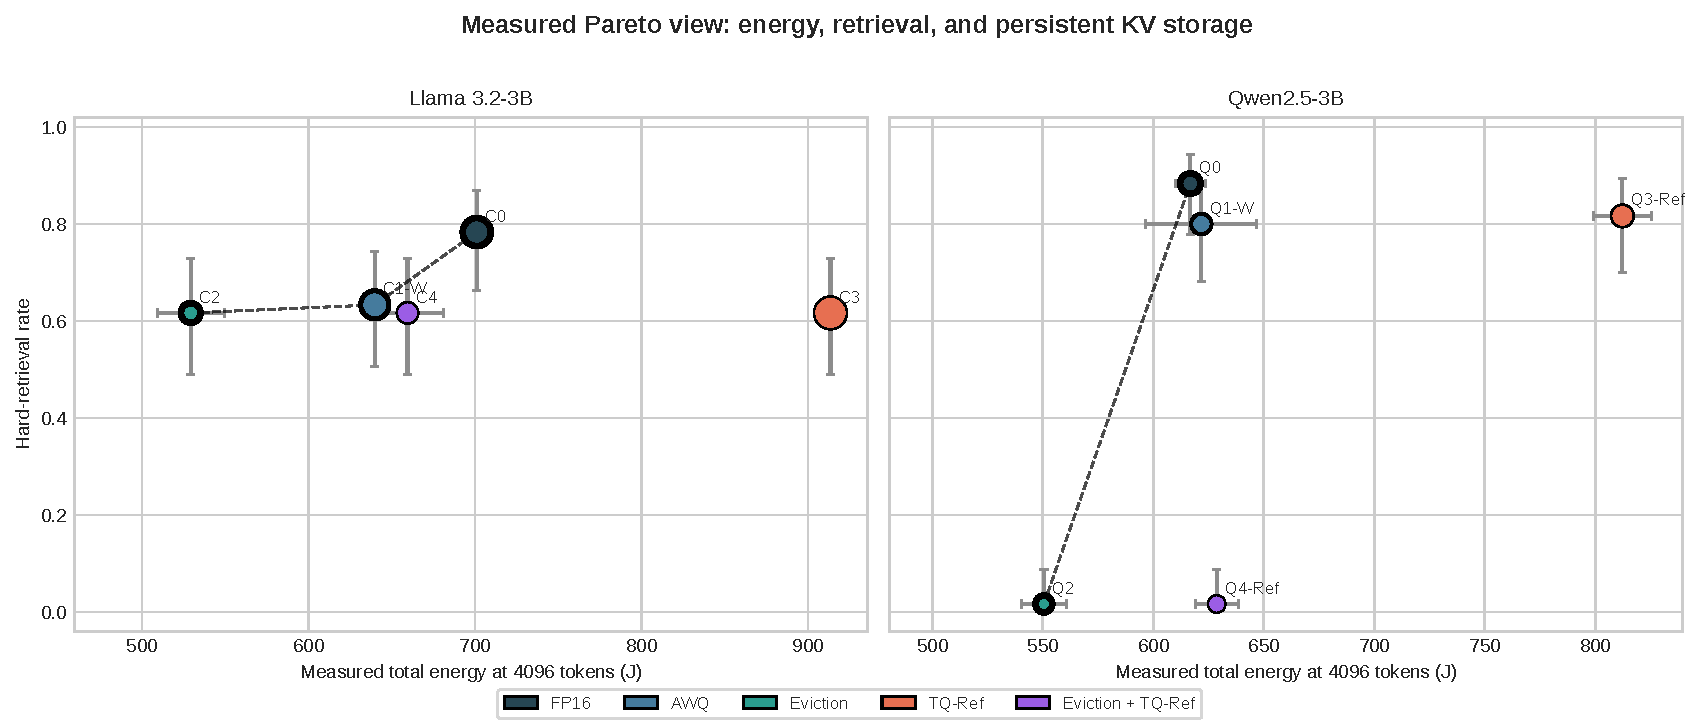
\includegraphics[width=\textwidth]{figures/fig08_measured_pareto_energy_quality_memory.pdf}
\Description{Two Pareto plots compare energy, retrieval quality, and persistent cache storage for Llama and Qwen at 4096 tokens.}
\caption{Measured energy--quality--memory Pareto view at 4096 tokens. Each marker
shows one configuration; marker area encodes persistent KV storage (bigger = more
memory); horizontal bars show energy SD; vertical bars show Wilson quality
intervals; edge width encodes bootstrap frontier-selection stability. Left: Llama.
Right: Qwen. The Qwen panel shows the stark separation between eviction (very low
energy, near-zero quality) and TQ-Ref (high energy, high quality).}
\label{fig:pareto3obj}
\end{figure*}

For Llama, C2 is the most compelling measured point: the lowest Llama energy
(529.30~J), the smallest persistent cache (119~MiB), and hard retrieval only one
scenario below the C1-W baseline (37/60 vs.\ 38/60). C0 and C1-W are also
frontier members (bootstrap frequency 100\% and 63\%), so C2 is not unique; it
is attractive because it achieves the lowest energy at a quality cost of only one
scenario. C3 and C4 were never or rarely selected (0\% and 0.6\%) because TQ-Ref
raised both energy and storage without improving hard retrieval.

For Qwen, the front separates into two incompatible regions: Q0 is the strongest
high-quality measured point (0.883 retrieval; 97.2\% bootstrap frequency), while
Q2 was always selected on energy and storage (100\%) but fails any minimum-quality
constraint (1/60 retrieval). Q3-Ref was rarely selected (3.8\%) because its high
energy dominates its quality advantage over Q1-W.

Bootstrap frontier frequency is resampling selection stability, not the probability
that a configuration is truly optimal. Pareto membership alone is not a deployment
recommendation; a minimum-quality constraint is required before any configuration
is selected.

\begin{table}[htbp]
\caption{Three-Objective Pareto Frontier at 4096 Tokens (2000 Bootstrap Resamples)}
\label{tab:pareto3}
\centering\small
\resizebox{\columnwidth}{!}{%
\begin{tabular}{@{}llrrrl@{}}
\toprule
\textbf{Model} & \textbf{Config} & \textbf{Energy (J)} & \textbf{Retrieval} & \textbf{Cache (MiB)} & \textbf{Boot.\%} \\
\midrule
Llama & C0     & 701.08 & 0.783 & 455 & 100.0\% \\
Llama & C1-W   & 639.86 & 0.633 & 455 &  63.0\% \\
Llama & C2     & 529.30 & 0.617 & 119 & 100.0\% \\
Llama & C3     & 913.48 & 0.617 & 697 &   0.0\% \\
Llama & C4     & 659.50 & 0.617 & 187 &   0.6\% \\
\midrule
Qwen  & Q0     & 616.78 & 0.883 & 146 &  97.2\% \\
Qwen  & Q1-W   & 621.75 & 0.800 & 146 &  36.0\% \\
Qwen  & Q2     & 550.48 & 0.017 &  38 & 100.0\% \\
Qwen  & Q3-Ref & 812.28 & 0.817 & 224 &   3.8\% \\
Qwen  & Q4-Ref & 628.69 & 0.017 &  60 &   0.0\% \\
\bottomrule
\end{tabular}}
\begin{minipage}{\columnwidth}\vspace{2pt}\footnotesize
Boot.\%: percentage of 2000 bootstrap resamples in which the configuration was
selected as a Pareto-optimal point. Higher means more stable frontier membership.
\end{minipage}
\end{table}

\subsection{Power Robustness: Are the Results Reliable?}
\label{sec:robustness}

The raw NVML traces contained power samples above the nominal 70~W enforced limit,
with some isolated values above 100~W and one at 124.5~W. We reintegrated all 100
Llama traces with samples above 82~W clipped, and then with samples above 70~W
clipped.

\begin{figure}[htbp]
\centering
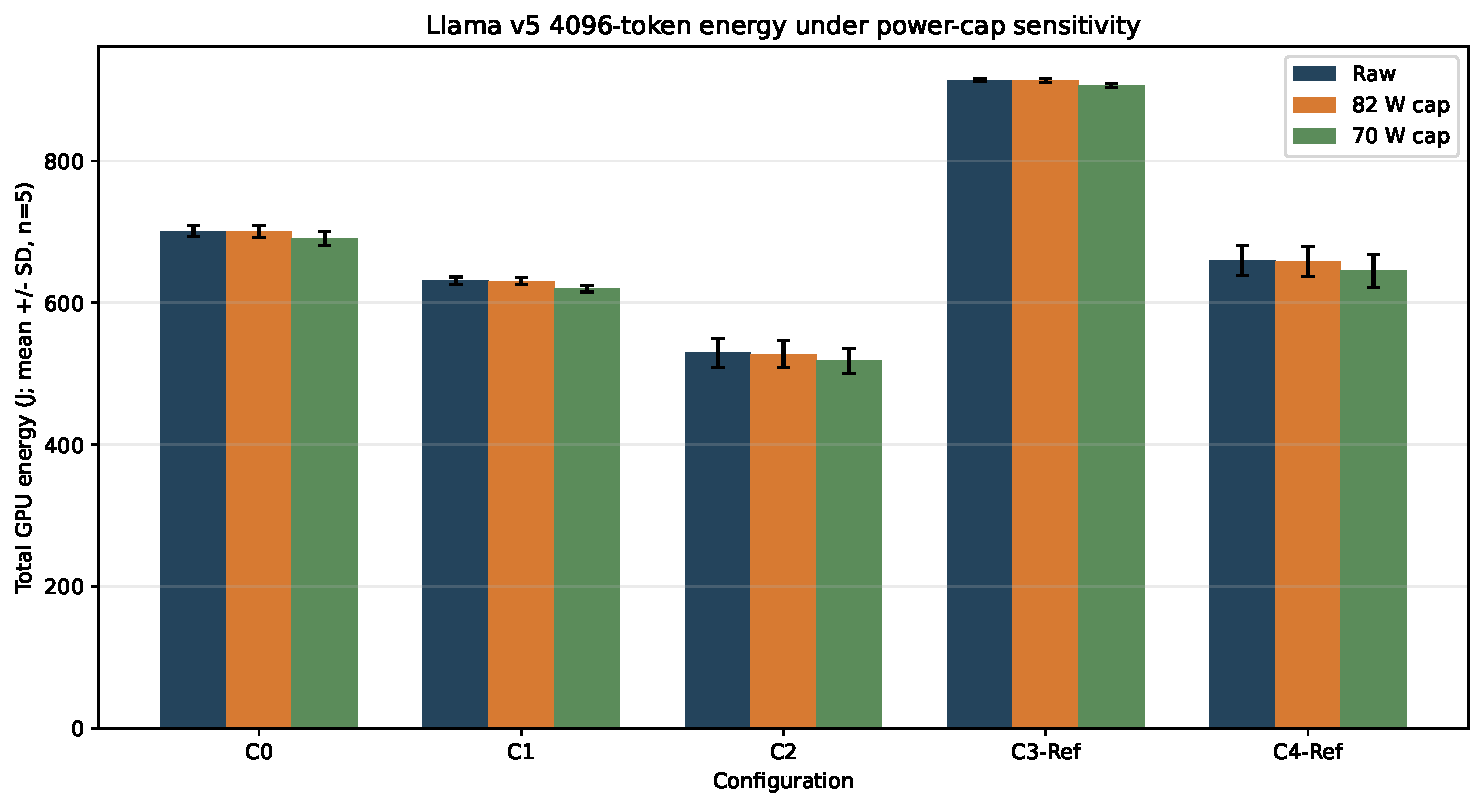
\includegraphics[width=\columnwidth]{figures/core_4096_power_cap_robustness.pdf}
\Description{A bar chart compares Llama total GPU energy under raw, 82-watt-clipped, and 70-watt-clipped trace integration.}
\caption{Total GPU energy at 4096 tokens for Llama: raw (dark), 82~W clip
(orange), and 70~W clip (green). All three bars maintain the same ordering
(C2~$<$~C1~$<$~C4~$<$~C0~$<$~C3). Energy differences from clipping are small
relative to between-configuration differences.}
\label{fig:power-cap}
\end{figure}

\begin{figure}[htbp]
\centering
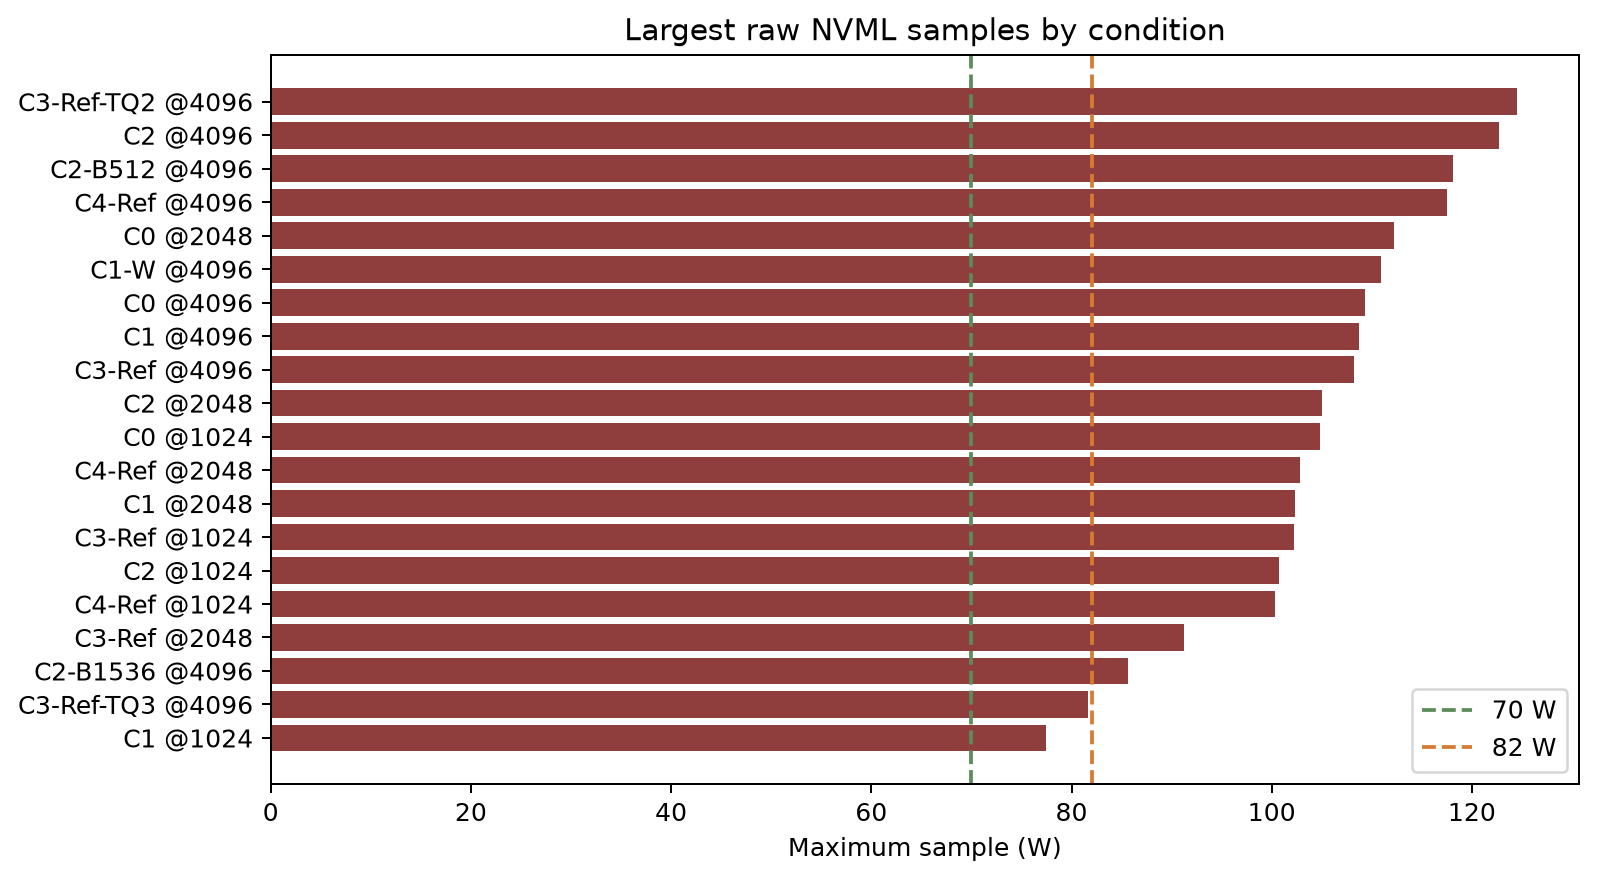
\includegraphics[width=\columnwidth]{figures/maximum_power_samples.png}
\Description{A sorted plot of maximum NVML power samples marks 70-watt and 82-watt thresholds and shows isolated samples above 100 watts.}
\caption{Maximum NVML sample (W) per condition, sorted. Dashed lines show the
70~W (green) and 82~W (orange) thresholds. Many conditions exceeded 100~W in at
least one sample; the highest recorded was 124.5~W.}
\label{fig:power-samples}
\end{figure}

Figures~\ref{fig:power-cap} and~\ref{fig:power-samples} show the result: all
three power regimes give the same energy ordering, and all five registered
significance decisions were unchanged. Power transients exist but do not change
the conclusions.

\subsection{Sensitivity: Budget and Bit Width}

\begin{figure}[htbp]
\centering
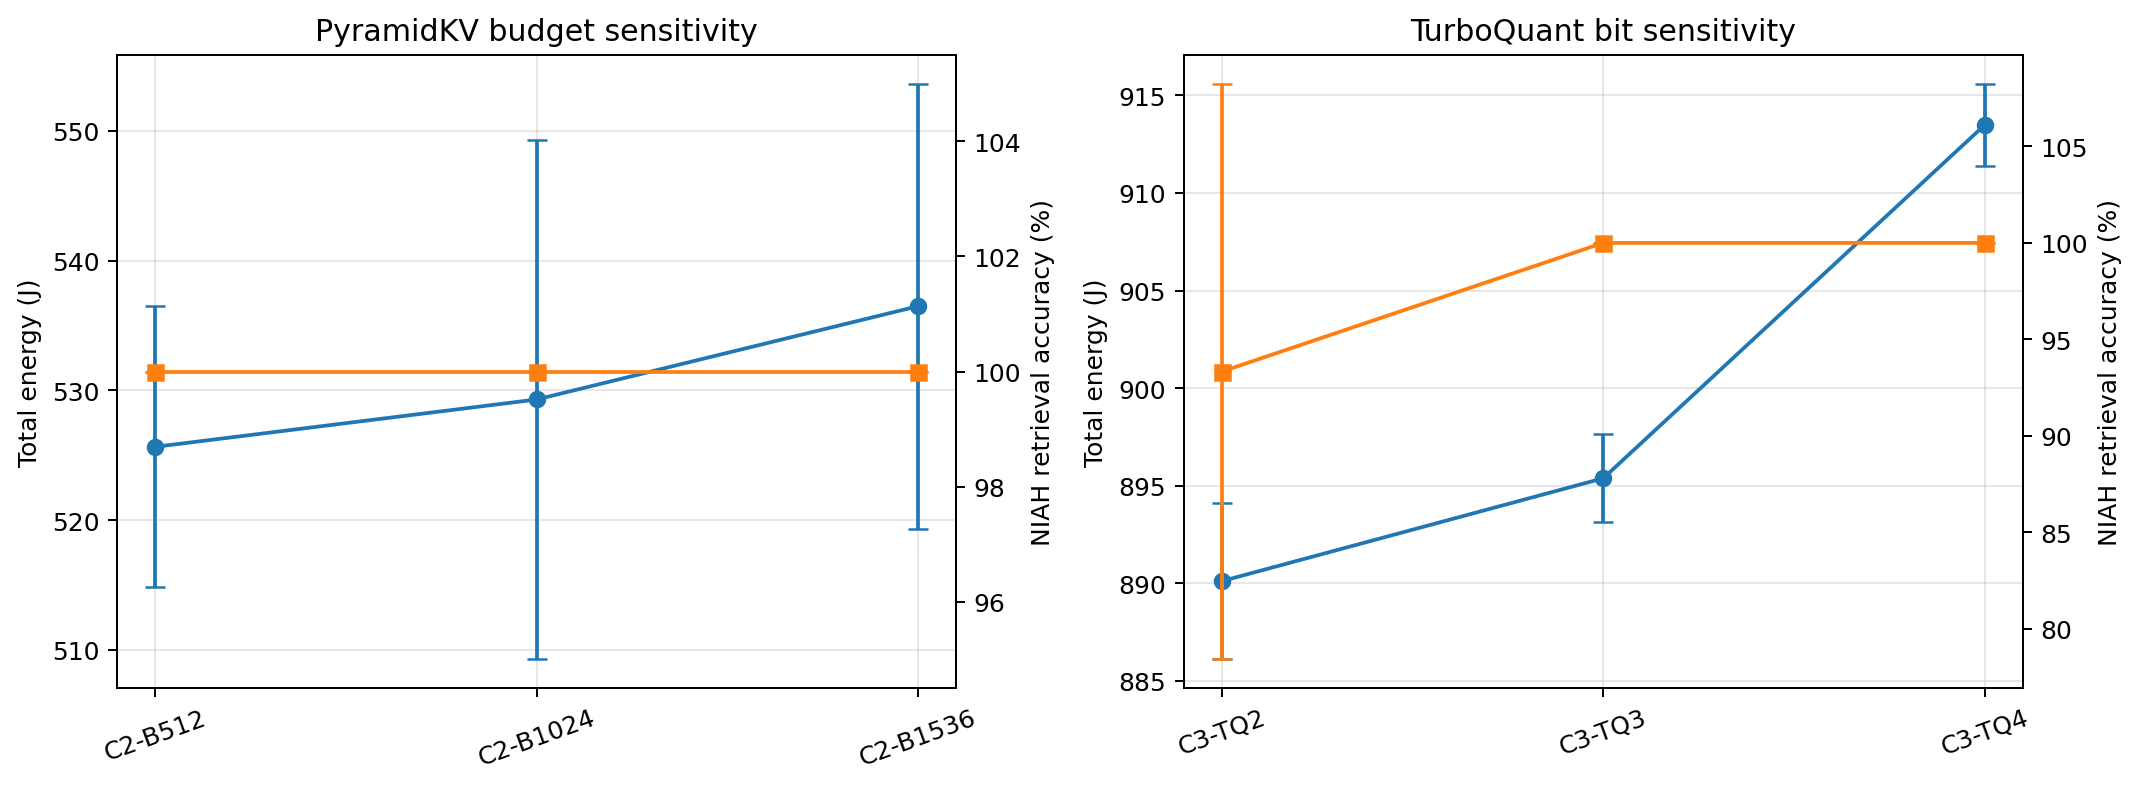
\includegraphics[width=\columnwidth]{figures/v5_final_sensitivity_4096.png}
\Description{Two plots show Llama energy and quality sensitivity to PyramidKV budget and TQ-Ref nominal bit width at 4096 tokens.}
\caption{Left: PyramidKV budget sensitivity for Llama at 4096 tokens (historical
easy-task benchmark; quality ceiling applies). Larger budgets cost slightly more
energy with no measurable quality change. Right: TQ-Ref nominal bit sensitivity
--- more bits cost more energy but improve quality. Note: energy is non-monotonic
across bit widths because all settings use uint8 physical storage.}
\label{fig:sensitivity}
\end{figure}

Qwen sensitivity is shown in Table~\ref{tab:qwen-sensitivity}: even at 1536
average retained tokens (50\% more than the main setting), eviction only recovered
2/15 scenarios, confirming the problem is not just budget level.

\subsection{Qwen Adapter Verification}
\label{sec:adapter}

Before running Qwen measurements, a parity pilot (Notebook~07) verified:
\begin{enumerate}
  \item Correct layer / head counts (36 layers, 16 Q heads, 2 KV heads).
  \item Stock AWQ (Q1-S) and wrapped AWQ (Q1-W) produced identical logits (zero
    difference).
  \item Pyramidal budget (avg 1024 tokens, range 1966--82 across 36 layers)
    correctly evicted tokens.
  \item TQ-Ref was numerically active with bounded reconstruction error
    (max normalized MSE $< 0.025$).
\end{enumerate}

This step produced zero measurement rows but is essential for reliability.

\subsection{Qwen: Energy Results}
\label{sec:qwen-energy}

Table~\ref{tab:qwen-all} shows Qwen's core energy results. The most notable
difference from Llama: AWQ (Q1-W) did not save energy compared to FP16 (Q0) at
any context. At 4096 tokens, Q0 averaged 616.78~J and Q1-W averaged 621.75~J
(essentially equal).

\begin{table}[htbp]
\caption{Qwen Energy (J, mean $\pm$ SD) at All Contexts}
\label{tab:qwen-all}
\centering\small
\resizebox{\columnwidth}{!}{%
\begin{tabular}{@{}lrrrrr@{}}
\toprule
\textbf{Context} & \textbf{Q0} & \textbf{Q1-W} & \textbf{Q2} & \textbf{Q3-Ref} & \textbf{Q4-Ref} \\
\midrule
1024 & $258.6\!\pm\!27.4$ & $293.4\!\pm\!21.6$ & $272.0\!\pm\!13.9$ & $358.6\!\pm\!9.6$  & $343.0\!\pm\!14.1$ \\
2048 & $334.2\!\pm\!17.5$ & $398.5\!\pm\!12.5$ & $342.6\!\pm\!10.3$ & $540.9\!\pm\!14.1$ & $435.2\!\pm\!20.0$ \\
4096 & $616.8\!\pm\!6.8$  & $621.8\!\pm\!25.1$ & $550.5\!\pm\!10.1$ & $812.3\!\pm\!13.1$ & $628.7\!\pm\!9.8$  \\
\bottomrule
\end{tabular}}
\end{table}

Q2 used the least energy at all three contexts. At 4096, Q2 saved 71.27~J
relative to Q1-W ($\approx$11.5\%), but Holm-corrected significance gave
$p = 0.0656$, narrowly above 0.05. This near-marginal result does not change the
conclusion: Q2's quality is essentially zero (Section~\ref{sec:qwen-quality}),
making its energy advantage practically unusable.

\subsection{Qwen: Hard-Retrieval Quality}
\label{sec:qwen-quality}

Table~\ref{tab:qwen-quality} shows Qwen's hard-retrieval results. The contrast
with Llama is dramatic.

\begin{table}[htbp]
\caption{Qwen Hard-Retrieval at 4096 Tokens (60 Scenarios)}
\label{tab:qwen-quality}
\centering\small
\begin{tabular}{lrrl}
\toprule
\textbf{Config} & \textbf{Pass/60} & \textbf{Rate} & \textbf{Wilson 95\% CI} \\
\midrule
Q0 (FP16)     & 53/60 & 0.883 & $[0.778,\ 0.942]$ \\
Q1-W (AWQ)    & 48/60 & 0.800 & $[0.682,\ 0.882]$ \\
Q2 (Evict)    & 1/60  & 0.017 & $[0.003,\ 0.089]$ \\
Q3-Ref (TQ)   & 49/60 & 0.817 & $[0.701,\ 0.894]$ \\
Q4-Ref (Both) & 1/60  & 0.017 & $[0.003,\ 0.089]$ \\
\bottomrule
\end{tabular}
\end{table}

Eviction (Q2) dropped retrieval to 1/60 across all depths (0/20, 0/20, 1/20).
The paired Q2-vs-Q1-W comparison had 47 losses and zero gains:
Bonferroni-adjusted McNemar $p \approx 1.71 \times 10^{-13}$. Q4-Ref also scored
1/60 --- following the eviction path, not the TQ-Ref path.

Q3-Ref preserved quality (49/60) with the same Wilson interval as Q1-W. It was
quality-preserving but energy-expensive: 190.53~J more than Q1-W at 4096 tokens
($+$30.6\%), a cost that remains meaningful when deployment is the goal.

\subsection{Cross-Model Retrieval Quality}

\begin{figure*}[htbp]
\centering
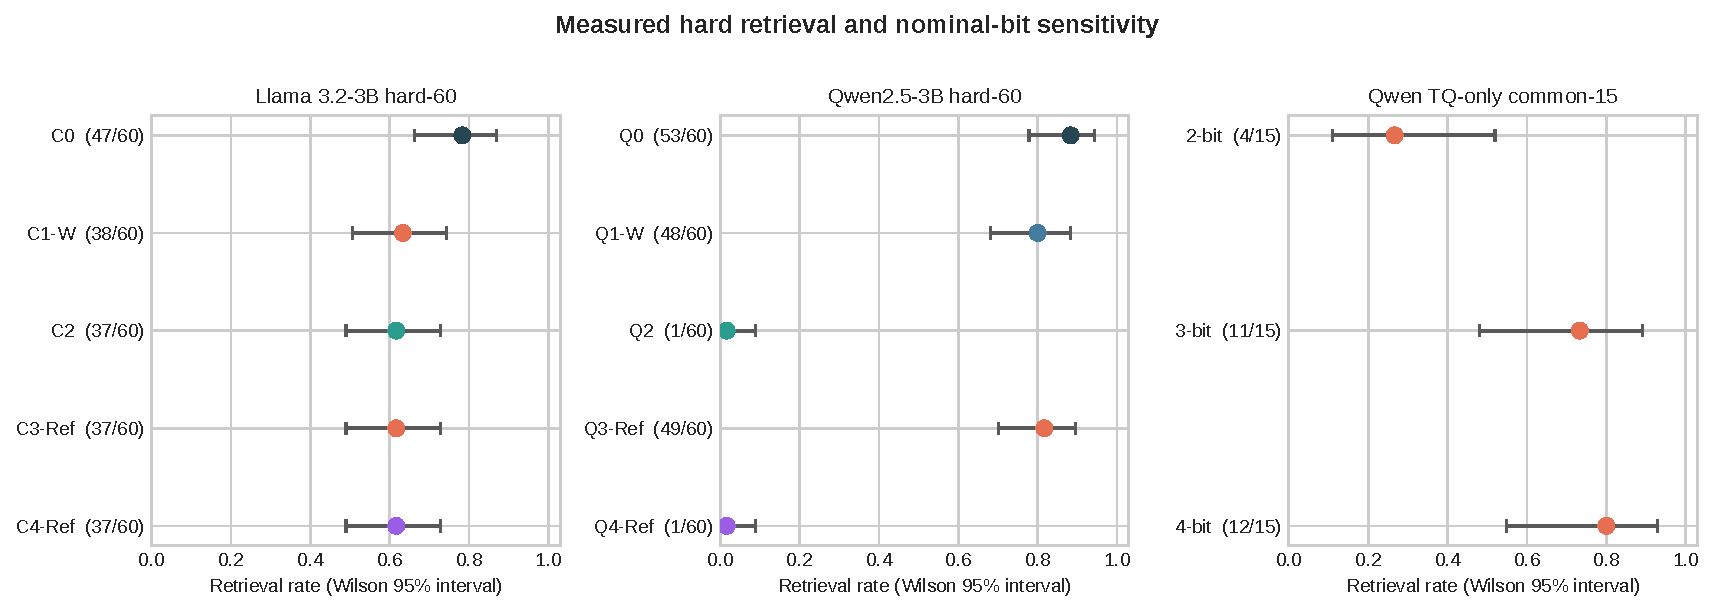
\includegraphics[width=\textwidth]{figures/fig03_retrieval_wilson.pdf}
\Description{Three plots show Wilson confidence intervals for Llama and Qwen retrieval rates and Qwen TQ bit-width sensitivity.}
\caption{Wilson-interval retrieval rates at 4096 tokens. Left: Llama hard-60 ---
all five configurations cluster near each other; C2/C3-Ref/C4-Ref each differ
from C1-W by only one scenario. Center: Qwen hard-60 --- Q2 and Q4-Ref collapse
near zero while Q3-Ref overlaps Q1-W. Right: Qwen common-15 TQ bit-width
sensitivity --- quality improves from 4/15 at 2~bits to 11/15 at 3~bits and
12/15 at 4~bits.}
\label{fig:wilson}
\end{figure*}

Figure~\ref{fig:wilson} puts the quality results side by side, making the
cross-model difference immediately visible.

The cross-model eviction quality contrast was $-0.767$ (bootstrap 95\% CI:
$[-0.867, -0.667]$): Qwen's eviction dropped retrieval by 76.7 percentage points
more than Llama's. This is large and practically important, but it is only two
models with different architectures, tokenizers, and sessions. We cannot identify
the causal factor from this evidence alone.

\subsection{Qwen Sensitivity Analysis}

\begin{table}[htbp]
\caption{Qwen Sensitivity at 4096 Tokens (Common-15 Scenarios)}
\label{tab:qwen-sensitivity}
\centering\small
\resizebox{\columnwidth}{!}{%
\begin{tabular}{@{}lrrl@{}}
\toprule
\textbf{Variant} & \textbf{Energy (J)} & \textbf{Retrieval} & \textbf{Wilson 95\% CI} \\
\midrule
\multicolumn{4}{l}{\textit{PyramidKV budget sweep}} \\
Q2-B512  & $515.2 \pm 8.9$  & 0/15 & $[0.000,\ 0.218]$ \\
Q2-B1024 & $550.5 \pm 10.1$ & 1/15 & $[0.003,\ 0.234]$ \\
Q2-B1536 & $590.6 \pm 13.2$ & 2/15 & $[0.026,\ 0.320]$ \\
\midrule
\multicolumn{4}{l}{\textit{TQ-Ref bit-width sweep}} \\
Q3-Ref-TQ2 & $808.9 \pm 34.0$ & 4/15  & $[0.109,\ 0.520]$ \\
Q3-Ref-TQ3 & $791.3 \pm 19.6$ & 11/15 & $[0.480,\ 0.891]$ \\
Q3-Ref-TQ4 & $812.3 \pm 13.1$ & 12/15 & $[0.548,\ 0.930]$ \\
\bottomrule
\end{tabular}}
\end{table}

The budget sweep confirms that even 1536 average retained tokens (50\% more than
the main setting) recovered only 2/15 scenarios. The failure was not simply a
budget-too-small problem. The TQ bit-width sweep shows 2-bit quality was
substantially lower (4/15), while 3-bit and 4-bit were close. Energy was
non-monotonic across bit widths because all settings use uint8 physical storage.

\subsection{Storage: The TurboQuant Realization Gap}

\begin{figure*}[htbp]
\centering
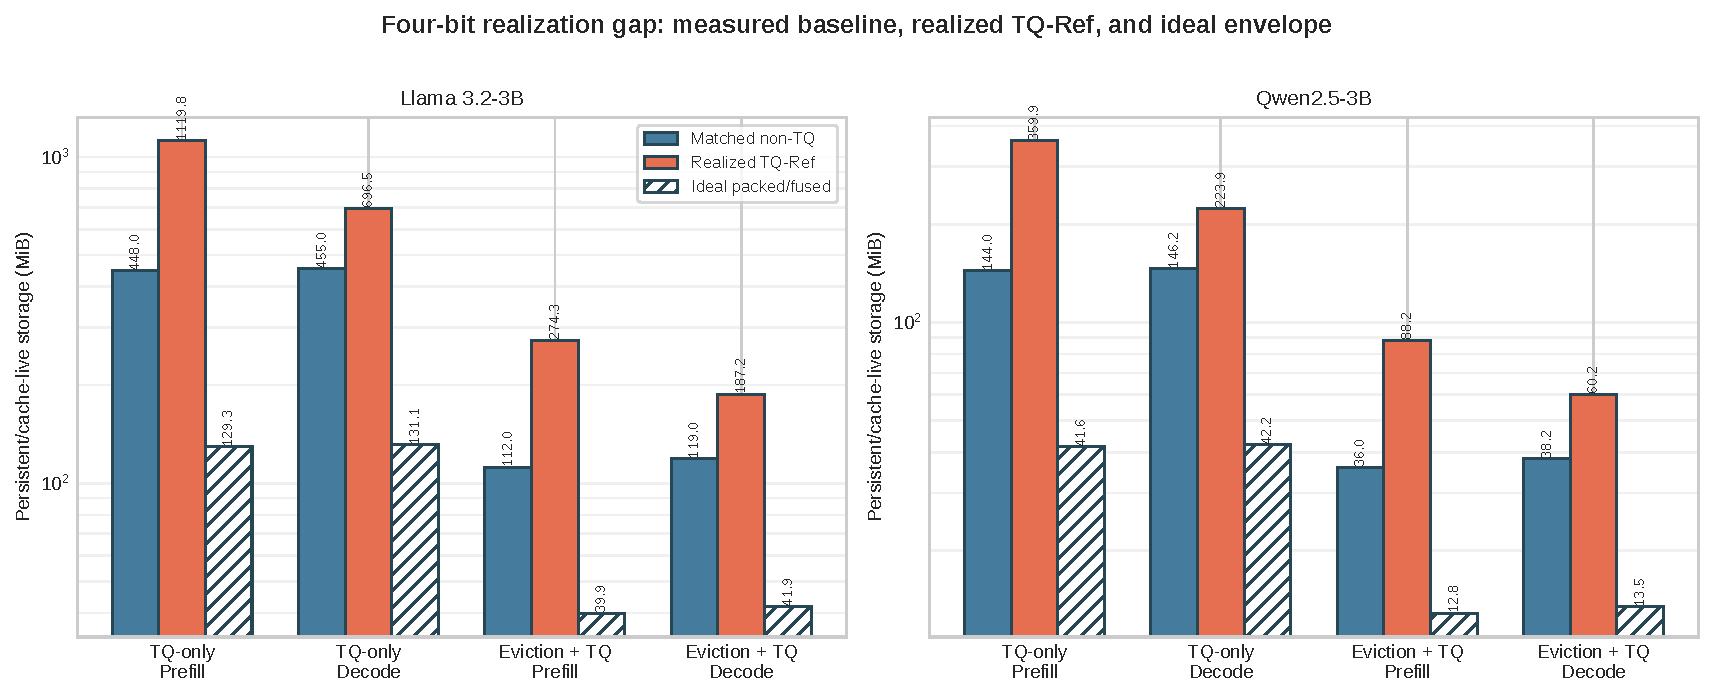
\includegraphics[width=\textwidth]{figures/fig04_storage_realization_gap.pdf}
\Description{A log-scale bar chart compares matched baseline, realized TQ-Ref, and ideal packed KV-cache storage for both models.}
\caption{Persistent KV cache storage for four-bit TQ paths (log axis). Blue bars
= matched non-TQ baseline; orange bars = realized TQ-Ref (larger because
materialized K/V is retained alongside uint8 indices); hatched bars = ideal
packed/fused layout (theoretical estimate). Realized storage is always larger
than matched non-TQ for both models. Ideal values are theoretical estimates, not
measurements.}
\label{fig:storage}
\end{figure*}

Figure~\ref{fig:storage} is the clearest illustration of why the TurboQuant
reference path is not a memory-saving solution in its current form. The orange
bars (realized storage) are always larger than the blue bars (baseline). The
hatched bars show what a future implementation could achieve if it truly packed
indices at the nominal bit width and discarded the materialized K/V tensors.

As shown in Figure~\ref{fig:tq_realization}, this difference arises because the
reference path retains materialized K/V tensors alongside its quantization state.

\begin{figure*}[htbp]
\centering
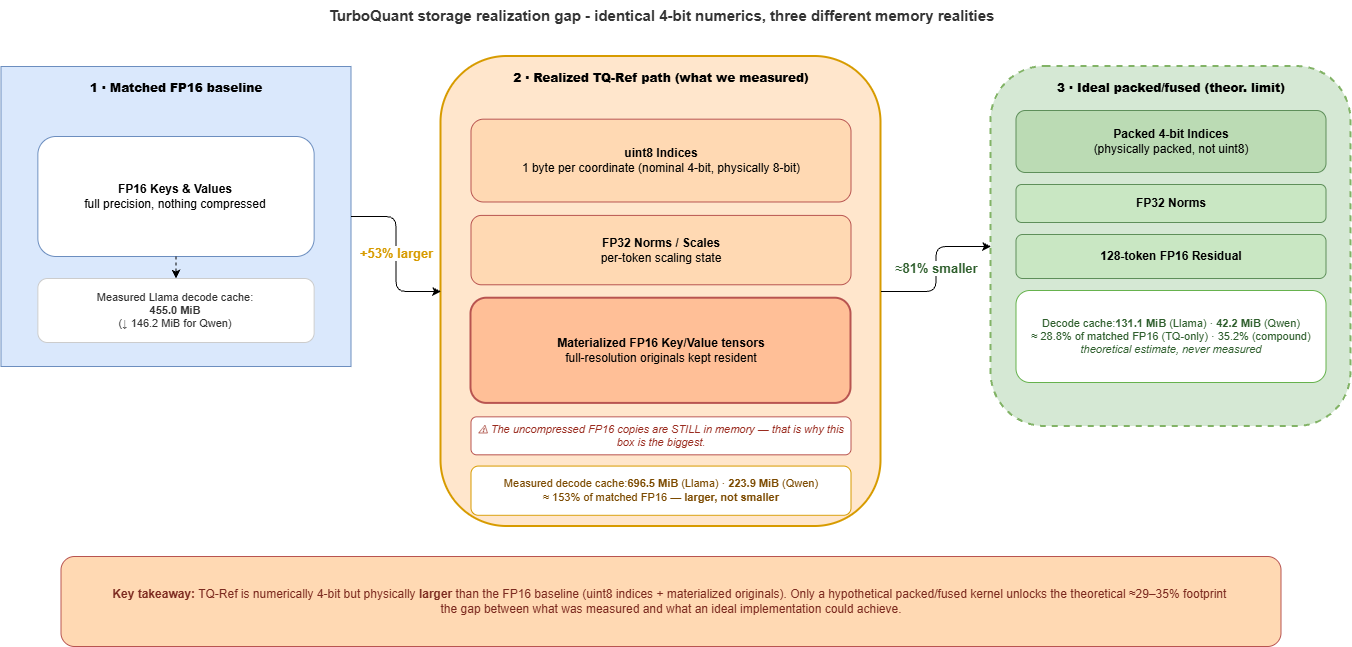
\includegraphics[width=\textwidth]{figures/turboquant_realization.png}
\Description{A diagram contrasts the measured TurboQuant reference path, which retains FP16 key-value tensors with quantization indices, against an ideal packed and fused path with reduced storage.}
\caption{The TurboQuant storage realization gap at 4-bit precision. The measured TQ-Ref path increases persistent VRAM usage by retaining materialized FP16 K/V tensors alongside quantization indices, whereas an ideal packed/fused implementation would significantly reduce storage requirements.}
\label{fig:tq_realization}
\end{figure*}

Table~\ref{tab:storage} gives the exact decode numbers:

\begin{table}[htbp]
\caption{Decode Storage at 4096 Tokens: Measured vs.\ Ideal (MiB)}
\label{tab:storage}
\centering\small
\resizebox{\columnwidth}{!}{%
\begin{tabular}{@{}lrrrr@{}}
\toprule
\textbf{Path} & \textbf{Non-TQ base} & \textbf{Realized TQ-Ref} & \textbf{Ideal packed} & \textbf{Ideal/FP16} \\
\midrule
Llama TQ-only   & 455.00 & 696.50 & 131.14 & 28.8\% \\
Llama evict.+TQ & 119.00 & 187.25 &  41.89 & 35.2\% \\
Qwen TQ-only    & 146.25 & 223.88 &  42.15 & 28.8\% \\
Qwen evict.+TQ  &  38.25 &  60.19 &  13.46 & 35.2\% \\
\bottomrule
\end{tabular}}
\begin{minipage}{\columnwidth}\vspace{2pt}\footnotesize
Ideal values are theoretical estimates assuming packed indices at nominal bit
width, FP32 norms, 128-token FP16 residual, and fused reconstruction. No such
implementation was measured.
\end{minipage}
\end{table}


%% ════════════════════════════════════════════════════════════════
%%  6. DISCUSSION
%% ════════════════════════════════════════════════════════════════
\section{Discussion}

\subsection{The Results Were Not What We Expected}

The original hypothesis was that stacking AWQ, eviction, and TurboQuant would
give a compound improvement: lower energy, lower memory, and preserved quality.
Table~\ref{tab:hypotheses} shows the divergence.

\begin{table}[htbp]
\caption{Original Hypotheses vs.\ Actual Findings}
\label{tab:hypotheses}
\centering\small
\resizebox{\columnwidth}{!}{%
\begin{tabular}{@{}p{0.44\columnwidth}p{0.52\columnwidth}@{}}
\toprule
\textbf{Expected} & \textbf{Actual} \\
\midrule
AWQ saves $\sim$3$\times$ energy & Only $\sim$10\% at 4096; costs more at 1024 \\
TQ reduces VRAM 15--20\% & Realized TQ-Ref \emph{increased} storage by 50\%+ \\
Eviction preserves retrieval & Llama: yes. Qwen: catastrophic failure (1/60) \\
Compound minimizes all objectives & C4 not significantly cheaper than C1; Q4 quality 1/60 \\
\bottomrule
\end{tabular}}
\end{table}

The divergence between expectation and outcome is itself a finding. Published
compression ratios come from ideal implementations; our measurements come from
actual reference code on a real GPU.

\subsection{Why Eviction Failed on Qwen but Not Llama}

The most surprising result is the eviction quality collapse on Qwen. We do not
know the exact cause. Possible reasons:
\begin{itemize}
  \item Qwen's 8:1 GQA ratio (2 KV heads for 16 query heads) versus Llama's 3:1
    ratio. The eviction scorer may behave differently when each KV head is shared
    by 8 query heads.
  \item Tokenizer-specific 4096-token materialization produced different byte
    sequences, potentially placing important context at positions the scorer ranked
    low.
  \item Our custom scorer was developed and validated primarily on Llama.
\end{itemize}

The budget sensitivity sweep showed that increasing from 512 to 1536 average
retained tokens only recovered 2/15 scenarios, suggesting the problem is in
\emph{which} tokens are discarded, not how many.

As shown in Figure~\ref{fig:eviction_gqa}, Qwen's more aggressive GQA sharing
means an eviction decision can remove context used by substantially more query
heads than in Llama.

\begin{figure*}[htbp]
\centering
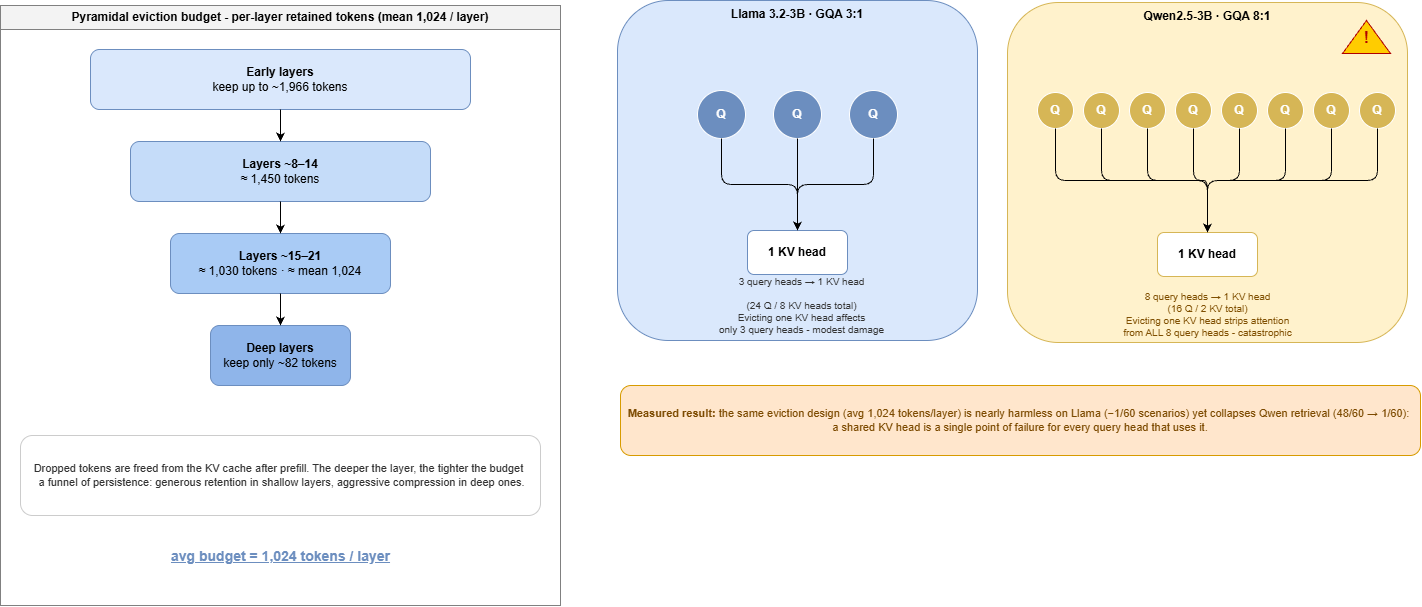
\includegraphics[width=\textwidth]{figures/eviction_graph.png}
\Description{A diagram compares pyramidal eviction budgets and grouped-query attention geometry: Llama shares each KV head with three query heads, while Qwen shares each KV head with eight query heads.}
\caption{Pyramidal eviction budget distribution alongside Grouped-Query Attention (GQA) geometries. Qwen's aggressive 8:1 GQA ratio creates a vulnerability where evicting one KV head strips context from eight query heads simultaneously, explaining its catastrophic retrieval collapse compared to Llama's 3:1 architecture.}
\label{fig:eviction_gqa}
\end{figure*}

\subsection{TurboQuant: Nominal vs.\ Physical}

Our TQ-Ref measurements are evidence about the reference path, not about an
optimized packed kernel. A production implementation that truly packs indices and
fuses reconstruction into the attention computation could potentially achieve the
ideal storage values in Table~\ref{tab:storage}. But we cannot claim savings that
were not observed. We think this distinction matters more than reporting
impressive-looking theoretical ratios.

\subsection{What the Statistics Do and Do Not Prove}

The registered evidence establishes:
\begin{enumerate}
  \item Llama eviction significantly reduces long-context energy (Holm $p = 0.00549$).
  \item TQ-Ref significantly increases energy on both models.
  \item Both models show significant negative sequential energy interactions
    (eviction shields TQ overhead, $p < 0.01$).
  \item Qwen eviction catastrophically degraded hard retrieval
    ($p \approx 10^{-13}$).
  \item All energy rankings and significance decisions were stable under 82~W and
    70~W power-trace clipping.
\end{enumerate}

The evidence does \emph{not} establish:
\begin{itemize}
  \item That C1-W and C4-Ref have exactly equal energy (the CI $[-60, 4]$~J
    crosses zero but is wide).
  \item That Qwen eviction failure was caused by GQA ratio or any specific
    mechanism.
  \item That TQ-Ref overhead would persist in a packed/fused implementation.
  \item That Llama results generalize to harder tasks or longer contexts.
  \item That AWQ uniformly saves energy at all context lengths.
\end{itemize}

\subsection{The Theoretical Limits of Sequential Stacking}

Recent theoretical frameworks highlight that strictly sequential compression pipelines are mathematically suboptimal compared to joint optimization strategies. As demonstrated by RDKV~\cite{zhang_rdkv_2026}, KV cache compression is fundamentally a rate-distortion bit allocation problem, where eviction is simply the zero-bit endpoint of a continuous precision curve. Unified methods solve this by using reverse water-filling algorithms to dynamically trade off token retention and precision in a single solver, allowing borderline tokens to be retained at lower bit-widths rather than being entirely discarded. Similarly, ThinKV~\cite{ramachandran_thinkv_2026} introduces thought-adaptive bit allocation to jointly couple quantization and eviction to the intrinsic importance of reasoning steps. A strictly sequential pipeline inherently lacks this dynamic flexibility. By enforcing rigid, isolated stages---first a binary keep-or-drop eviction, followed by fixed quantization of the survivors---sequential stacking prevents flexible precision allocation and risks compounding approximation errors downstream.

Despite these mathematical limitations, our empirical hardware findings reveal a different operational reality. Our data proves that sequential stacking provides a highly practical, physical ``energy shield'' on edge hardware. By aggressively filtering tokens before they reach the quantization step, the sequential approach actively masks the massive computational overhead of unfused quantization kernels, which currently bottleneck real-world edge deployment.


%% ════════════════════════════════════════════════════════════════
%%  7. THREATS TO VALIDITY
%% ════════════════════════════════════════════════════════════════
\section{Threats to Validity}

\subsection{Internal Validity}
Each model's core measurement matrix was collected in one Colab session. We
collected five energy blocks per condition, giving enough power for large effects
but not for small ones. The Llama systems matrix used stock AWQ (C1) as the
baseline while compressed paths (C2--C4) used a custom wrapper, introducing a
small wrapper overhead ($\approx$8.61~J at 4096). Qwen used the matched wrapper
throughout. Notebook~08 required two in-session code repairs, preserved inline;
raw measurements are hash-verified and were not recollected.

\subsection{Construct Validity}
Hard retrieval using exact code extraction at three depths measures one type of
quality. Open-ended generation, reasoning, summarization, and multilingual tasks
may behave differently. Energy is GPU board power (NVML) and does not include CPU,
host DRAM, or cooling overhead.

\subsection{External Validity}
We tested exactly two models on one GPU. The eviction results were completely
different between models. Results from one model cannot be assumed to hold for
another. All experiments used Google Colab free tier, which does not guarantee
consistent hardware assignment. Teacher-forced 64-token decode is not the same as
open-ended generation.

\subsection{Statistical Conclusion Validity}
Holm correction was applied within each test family. Wilson intervals at $n = 60$
span roughly $\pm$13 percentage points; the $n = 15$ sensitivity intervals are
much wider ($\pm$20+ pp). Bootstrap Pareto frequency measures resampling stability,
not true optimality probability.


%% ════════════════════════════════════════════════════════════════
%%  8. CONCLUSION
%% ════════════════════════════════════════════════════════════════
\section{Conclusion}

This paper measured three stacked compression methods on two 3B language models
running on an NVIDIA T4, using real GPU power traces and a carefully calibrated
hard-retrieval benchmark. The results show that:

\begin{enumerate}
  \item \textbf{Eviction (C2/Q2)} is the strongest measured energy trade-off at
    long context: it reduces energy by 12--16\% and dramatically shrinks KV cache
    size. But on Qwen, it destroyed retrieval quality (1/60 vs.\ 48/60 baseline).
    On Llama, retrieval changed by only one scenario.

  \item \textbf{TurboQuant reference (C3/Q3-Ref)} adds substantial energy overhead
    (31--45\%) because the current implementation keeps materialized K/V tensors
    alongside quantization state. Qwen's TQ-Ref preserved retrieval well (49/60)
    while Llama's was unchanged.

  \item \textbf{AWQ alone} saves energy only at long context ($\approx$10\% at
    4096 tokens); at short context it can cost more.

  \item \textbf{Sequential compound (C4/Q4-Ref)} shows that eviction shields
    TQ-Ref overhead (significant negative energy interaction on both models), but
    the compound path still inherits Qwen's eviction quality failure.

  \item \textbf{Pareto frontier with uncertainty} (Figure~\ref{fig:pareto3obj})
    shows that C2 is the most attractive measured Llama point: lowest energy,
    smallest persistent cache, and hard retrieval one scenario below baseline,
    with 100\% bootstrap frontier-selection frequency. It is not unique---C0 and
    C1-W are also frontier members---and Pareto membership alone is never a
    deployment recommendation: a minimum-quality constraint is required (Qwen's
    Q2 is always frontier-selected yet unusable at 1/60 retrieval).
\end{enumerate}

The clearest lesson is that compression results from one model do not transfer to
another without validation. Measuring real power on real hardware gives different
answers than published compression ratios might suggest. Future work should test
production-kernel implementations of TurboQuant, official KVCache-Factory eviction,
and more context lengths to build a more general picture.


%% ════════════════════════════════════════════════════════════════
%%  GENERATIVE AI USAGE STATEMENT
%% ════════════════════════════════════════════════════════════════
\section*{Generative AI Usage Statement}

Generative AI tools were used in the preparation of this work in two
capacities: (1)~\emph{code generation}—AI-assisted code suggestions were
used to accelerate the implementation of experiment notebooks, data
processing pipelines, and visualization scripts; and (2)~\emph{reference
matching and fact-checking}—AI tools were consulted to locate candidate
citations and to cross-check factual claims against source material. In
both cases, all AI-generated outputs were critically reviewed,
independently verified, and validated by the authors before incorporation
into the final work. No AI-generated text was accepted without human
scrutiny, and the intellectual content, experimental design, analysis, and
conclusions presented in this paper are entirely the work of the authors.

%% ════════════════════════════════════════════════════════════════
%%  REFERENCES
%% ════════════════════════════════════════════════════════════════
%% Print all BibTeX entries, including uncited background references.
\nocite{*}
\bibliographystyle{ACM-Reference-Format}
\begingroup
\sloppy
\hbadness=10000
\bibliography{references}
\endgroup

%% ════════════════════════════════════════════════════════════════
%%  APPENDIX: IDEAL PACKED/FUSED TQ ANALYSIS
%% ════════════════════════════════════════════════════════════════
\clearpage  %% flush all pending main-body floats before appendix
\appendix
\section{Ideal Packed/Fused TQ Analysis}
\label{app:ideal}

This appendix presents the mathematical ideal-layout analysis from Notebook~09.
All figures here are theoretical estimates, not experimental measurements. No numerical ideal
energy, latency, throughput, or peak-VRAM value is claimed.

\subsection{Ideal Storage Decomposition}

Figure~\ref{fig:ideal-components} shows how the four components of ideal storage
(packed indices, FP32 norms, FP16 residual, metadata) scale with bit width. Packed
indices grow with bit width; norms and residual are fixed for a given retained-token
structure. The normalized ratios match across Llama and Qwen because the model is
geometry-normalized, not claiming equal absolute bytes.

If a future implementation packs indices at the nominal bit width and removes
persistent materialized K/V, ideal decode storage ranges from $\approx$16.7\% of
FP16 at 2~bits to $\approx$28.8\% at 4~bits (TQ-only), or $\approx$24.2\% to
$\approx$35.2\% with prior eviction. The compound ratios are higher than
TQ-only because the fixed 128-token residual is a larger fraction of a smaller
evicted cache.

\subsection{Modeled Phase Byte Demand}

Figure~\ref{fig:phase-demand} models logical compulsory dataflow, not exact DRAM
transactions. Prefill cannot claim compressed attention reads because full-prompt
attention happens before eviction/quantized persistence. Packing introduces a
conversion read and compressed writes. Decode then repeatedly reads the growing
cache; a fused implementation can potentially avoid materialized reconstruction
writes.

\subsection{Symbolic Break-Even Boundary}

The ideal energy model is:
\begin{equation}
E_\text{ideal} = E_\text{baseline} - \epsilon_\text{mem} \cdot \Delta_D + O_\text{net}
\end{equation}
where $\epsilon_\text{mem}$ is the effective energy per avoided modeled byte and
$O_\text{net}$ includes rotation, packing, reconstruction compute, and control
overhead. When $\Delta_D > 0$ (decode savings), strict reduction requires
$O_\text{net} < \epsilon_\text{mem} \cdot \Delta_D$.

Figure~\ref{fig:break-even} plots the maximum allowable $O_\text{net}/\epsilon_\text{mem}$
for each path. The boundaries are largest for non-evicted 2-bit paths and smallest
for compound 4-bit paths. No finite values are assigned to either unknown; the
figure is a conditional reference, not an energy forecast.

\begin{figure*}[!t]
\centering
\begin{subfigure}{0.76\textwidth}
\centering
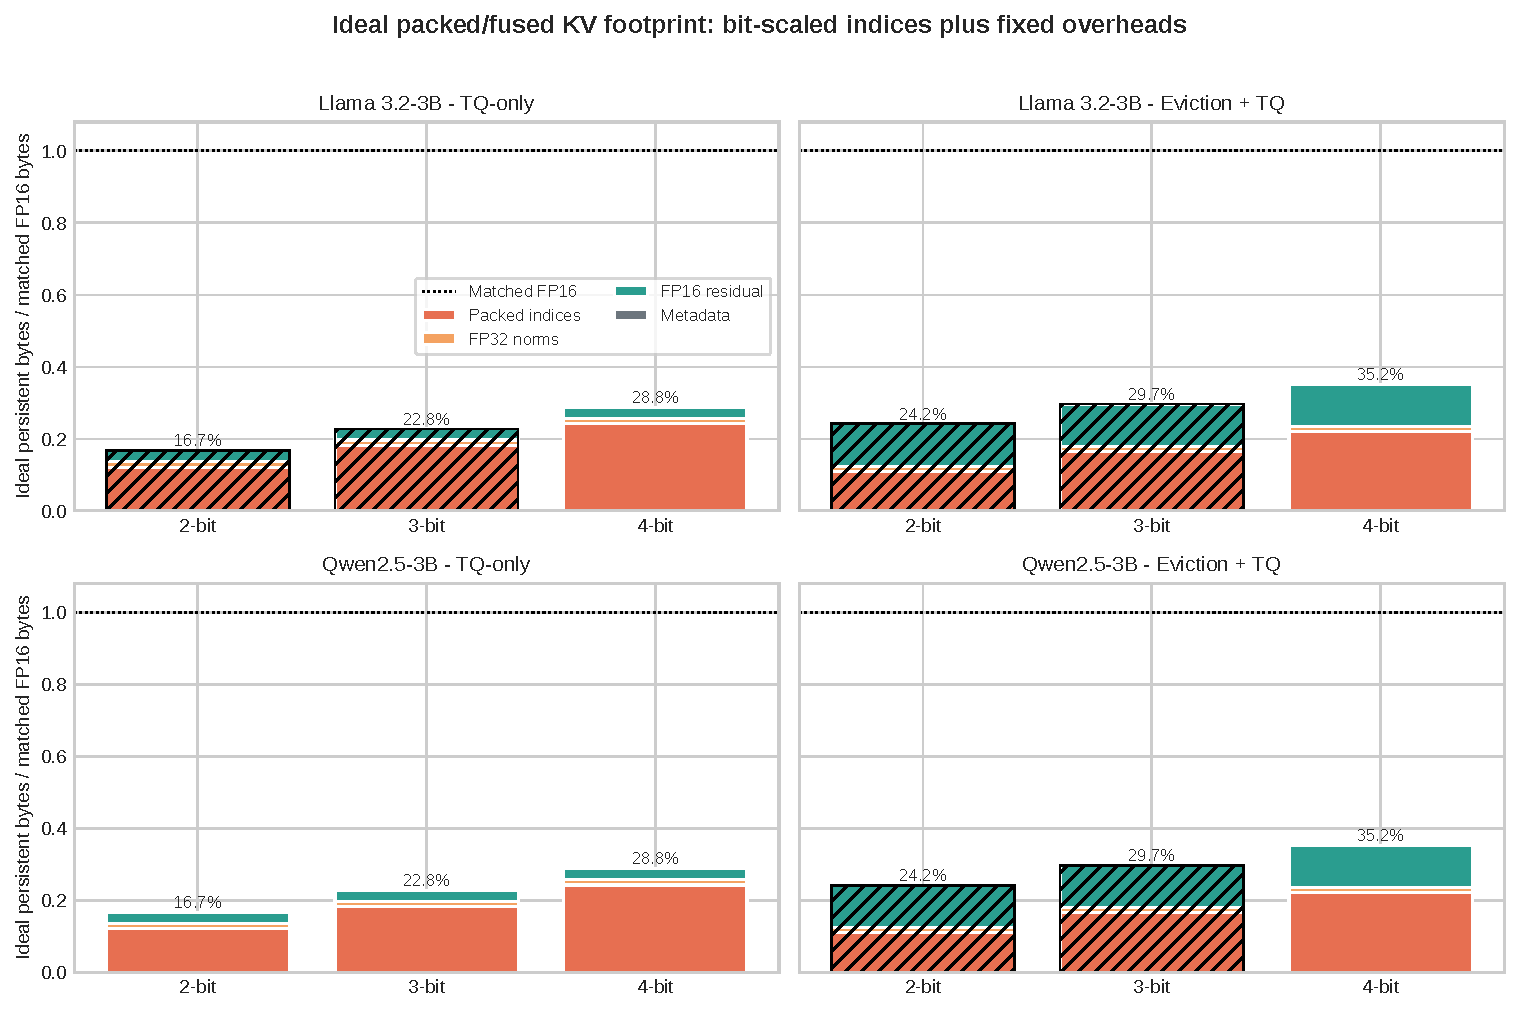
\includegraphics[width=\textwidth]{figures/fig05_ideal_packed_components.pdf}
\caption{Ideal packed/fused KV footprint, decomposed into packed indices, FP32 norms, FP16 residual, and metadata.}
\label{fig:ideal-components}
\end{subfigure}

\vspace{3pt}
\begin{subfigure}[t]{0.48\textwidth}
\centering
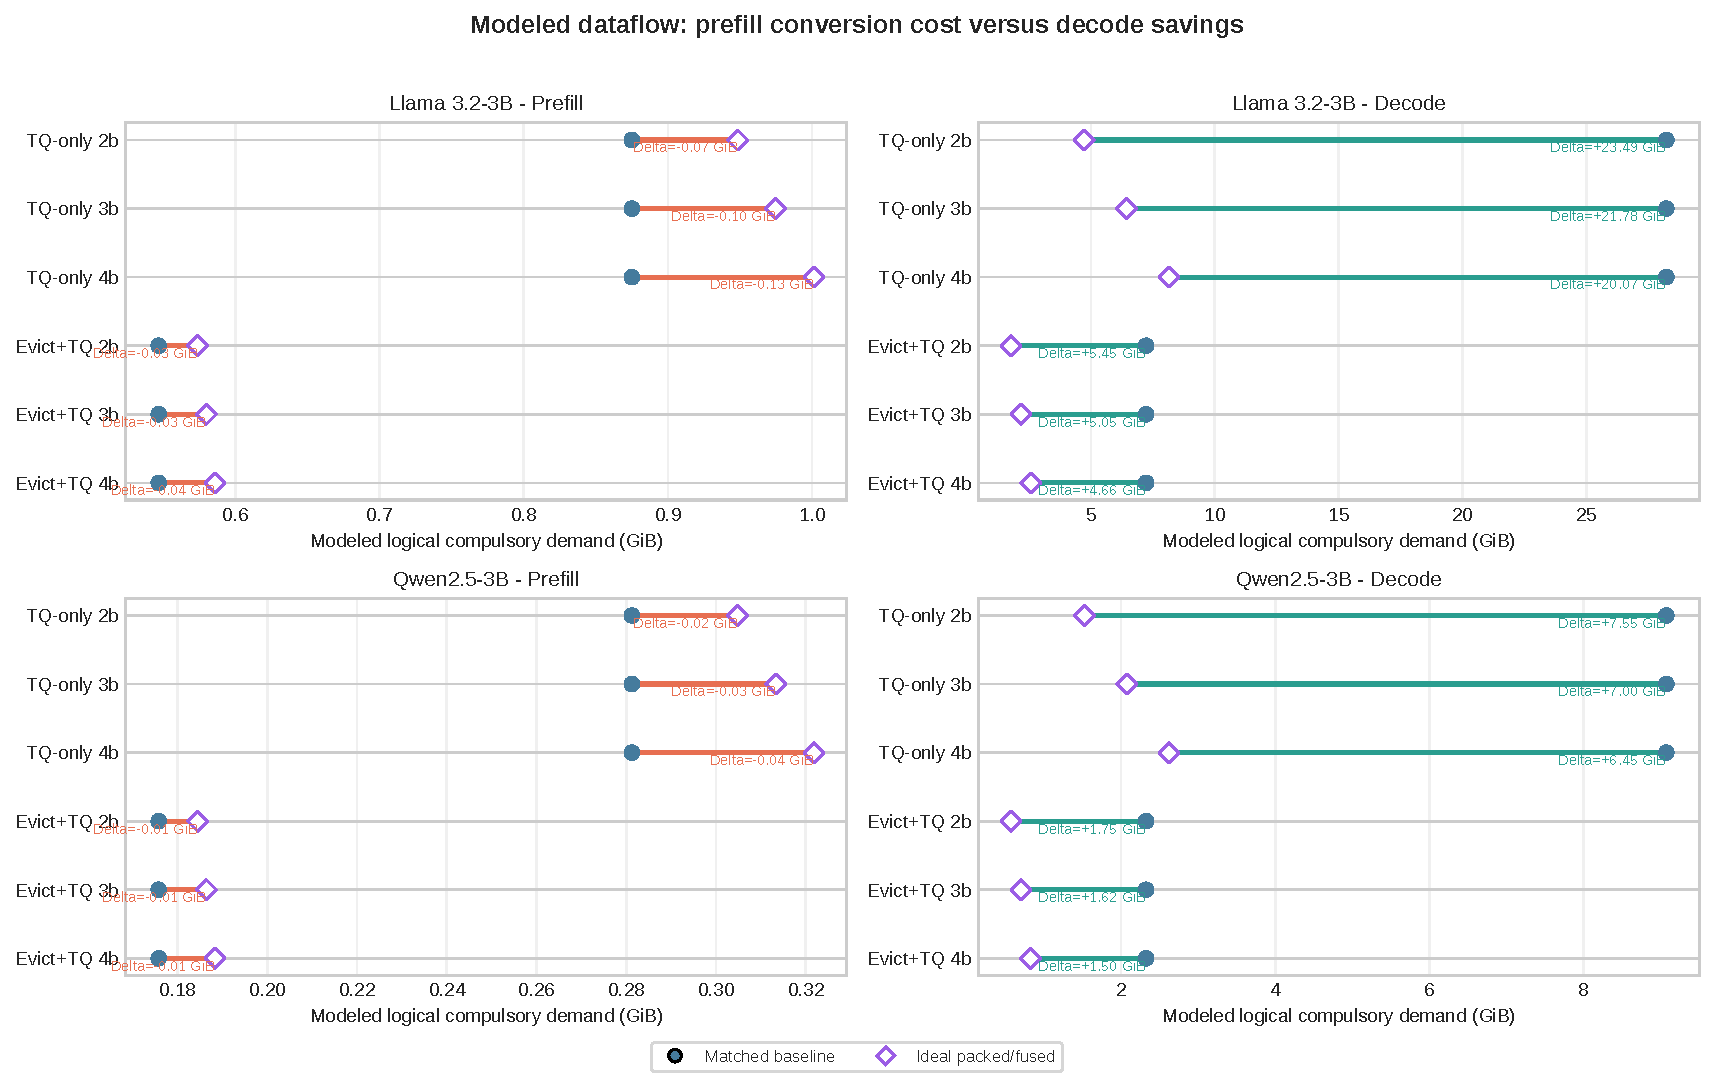
\includegraphics[width=\textwidth]{figures/fig06_modeled_phase_byte_demand.pdf}
\caption{Modeled compulsory dataflow for baseline and ideal packed/fused paths during prefill and decode.}
\label{fig:phase-demand}
\end{subfigure}\hfill
\begin{subfigure}[t]{0.48\textwidth}
\centering
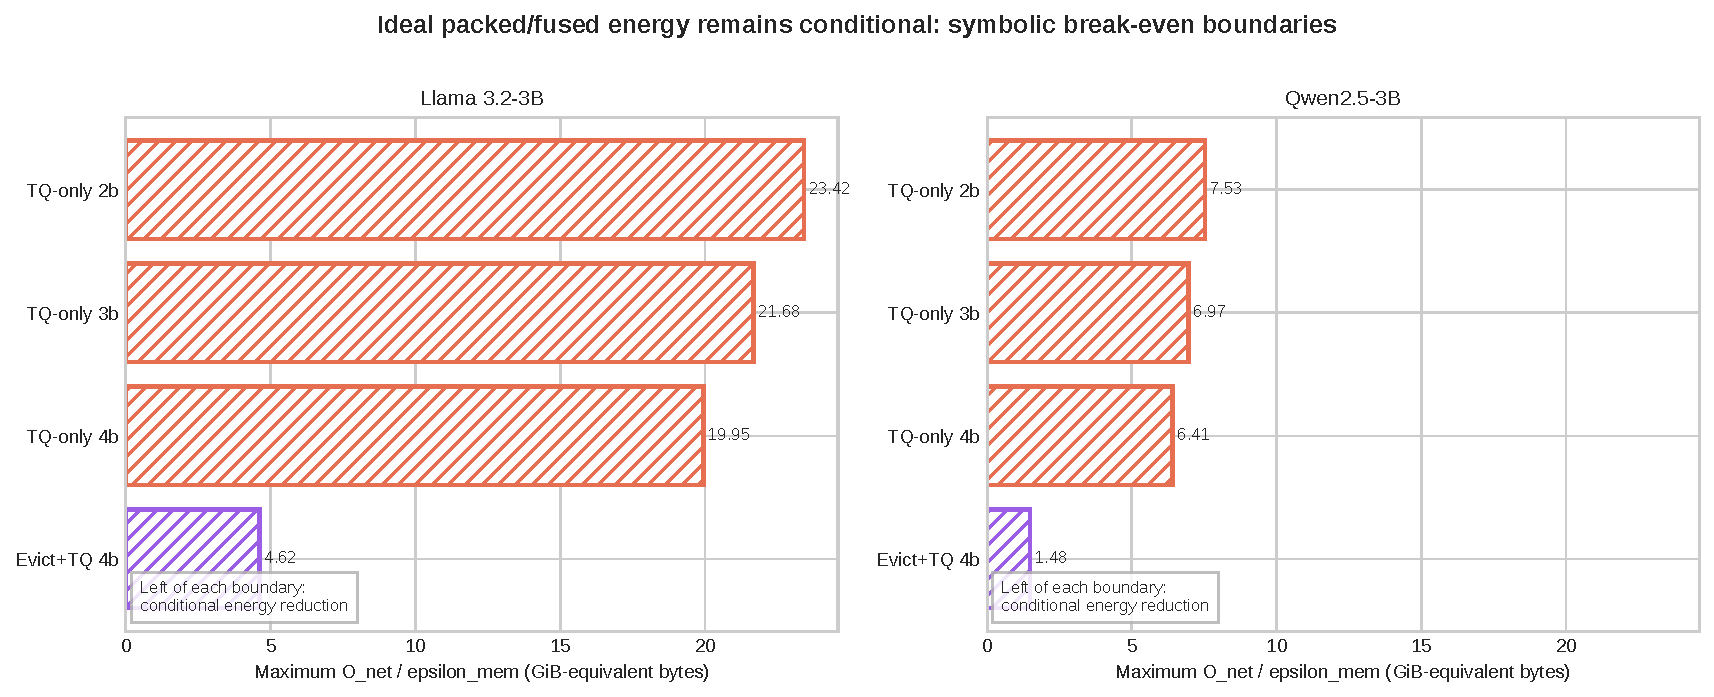
\includegraphics[width=\textwidth]{figures/fig07_symbolic_energy_break_even.pdf}
\caption{Symbolic break-even bounds for the ideal compressed KV-cache paths.}
\label{fig:break-even}
\end{subfigure}
\Description{Three appendix diagrams summarize ideal KV-cache compression: a footprint decomposition, modeled dataflow, and symbolic energy break-even bounds.}
\caption{Compact overview of the ideal packed/fused TurboQuant analysis. All values are theoretical estimates, not experimental measurements.}
\end{figure*}


\end{document}
